\documentclass[11pt]{report}
\bibliographystyle{ieeetr}
\usepackage[a4paper, total={6in, 8.15in}]{geometry}
\usepackage{caption} 
\captionsetup[table]{skip=5pt}
\usepackage{amsmath}
\usepackage{multirow}
\usepackage{booktabs}
\usepackage{pdflscape}
\usepackage{blindtext}
\usepackage{parskip}
\usepackage{tablefootnote}
\usepackage{enumitem}
\usepackage[nottoc,numbib]{tocbibind}
\usepackage[section]{placeins}
\usepackage{graphicx} % Required for inserting images
\usepackage[english]{babel}
\usepackage{pdfpages}
\usepackage{xargs}                      % Use more than one optional parameter in a new commands
\usepackage{nameref}
\usepackage[toc,page]{appendix}
\usepackage{titlesec}
\usepackage[acronym]{glossaries}
%\usepackage[pdftex,dvipsnames]{xcolor}  % Coloured text etc.
%
\interfootnotelinepenalty=10000
\usepackage[colorinlistoftodos,prependcaption,textsize=tiny]{todonotes}
\newcommandx{\unsure}[2][1=]{\todo[linecolor=red,backgroundcolor=red!25,bordercolor=red,#1]{#2}}
\newcommandx{\change}[2][1=]{\todo[linecolor=blue,backgroundcolor=blue!25,bordercolor=blue,#1]{#2}}
\newcommandx{\info}[2][1=]{\todo[linecolor=OliveGreen,backgroundcolor=OliveGreen!25,bordercolor=OliveGreen,#1]{#2}}
\newcommandx{\improvement}[2][1=]{\todo[linecolor=orange,backgroundcolor=orange!25,bordercolor=orange,#1]{#2}}
\newcommandx{\thiswillnotshow}[2][1=]{\todo[disable,#1]{#2}}

\usepackage{enumitem}
\usepackage[hyperref = true, only-used = false, list-style = longtable]{acro}
\usepackage{pdfcomment}
\usepackage{hyperref}
\newcommand*{\fullref}[1]{\hyperref[{#1}]{\autoref*{#1} \nameref*{#1}}}
\acsetup{
	make-links 		= 	false,
	pdfcomments/use		=	true,
}

\DeclareAcronym{VTC}{short = {VTC}, long = {Value-transfer chain}, pdfcomment = {Value-transfer chain}}

\DeclareAcronym{GPC}{short = {GPC}, long = {General-purpose chain}, pdfcomment = {General-purpose chain}}
%\DeclareAcronym{ESG}{short = {ESG}, long = {Environmental Social \& Governance}, pdfcomment = {Environmental Social \& Governance}}
\DeclareAcronym{CCRI}{short={CCRI}, long={Crypto Carbon Ratings Institute}, pdfcomment = {Crypto Carbon Ratings Institute}}

\DeclareAcronym{ESG}{short = {ESG}, long = {Environmental Social \& Governance}, pdfcomment = {Environmental Social \& Governance}
}

\DeclareAcronym{LCA}{ short = {LCA}, long = {Life Cycle Assessment}, pdfcomment = {Life Cycle Assessment}
}

\DeclareAcronym{GHG}{ short = {GHG}, long = {Greenhouse Gas}, pdfcomment = {Greenhouse Gas}
}

\DeclareAcronym{CO2e}{ short = {CO2e}, long = {Carbon Dioxide Equivalent}, pdfcomment = {Carbon Dioxide Equivalent}
}

\DeclareAcronym{DAO}{ short = {DAO}, long = {Decentralized Autonomous Organization}, pdfcomment = {Decentralized Autonomous Organization}
}

\DeclareAcronym{PoW}{short = {PoW},long = {Proof-of-Work},pdfcomment = {Proof-of-Work}
}

\DeclareAcronym{PoS}{ short = {PoS}, long = {Proof-of-Stake}, pdfcomment = {Proof-of-Stake}
}

\DeclareAcronym{EVM}{ short = {EVM}, long = {Ethereum Virtual Machine}, pdfcomment = {Ethereum Virtual Machine}
}

\DeclareAcronym{Tx}{ short = {Tx}, long = {Transaction}, pdfcomment = {Transaction}
}

\DeclareAcronym{DLT}{short = {DLT}, long = {Distributed Ledger Technology}, pdfcomment = {Distributed Ledger Technology}}


\parskip 2ex
\parindent 0pt

\title{GreenBlocks - SMT PdM}
\author{mbelanger.poly}
\date{August 2023}


\begin{document}

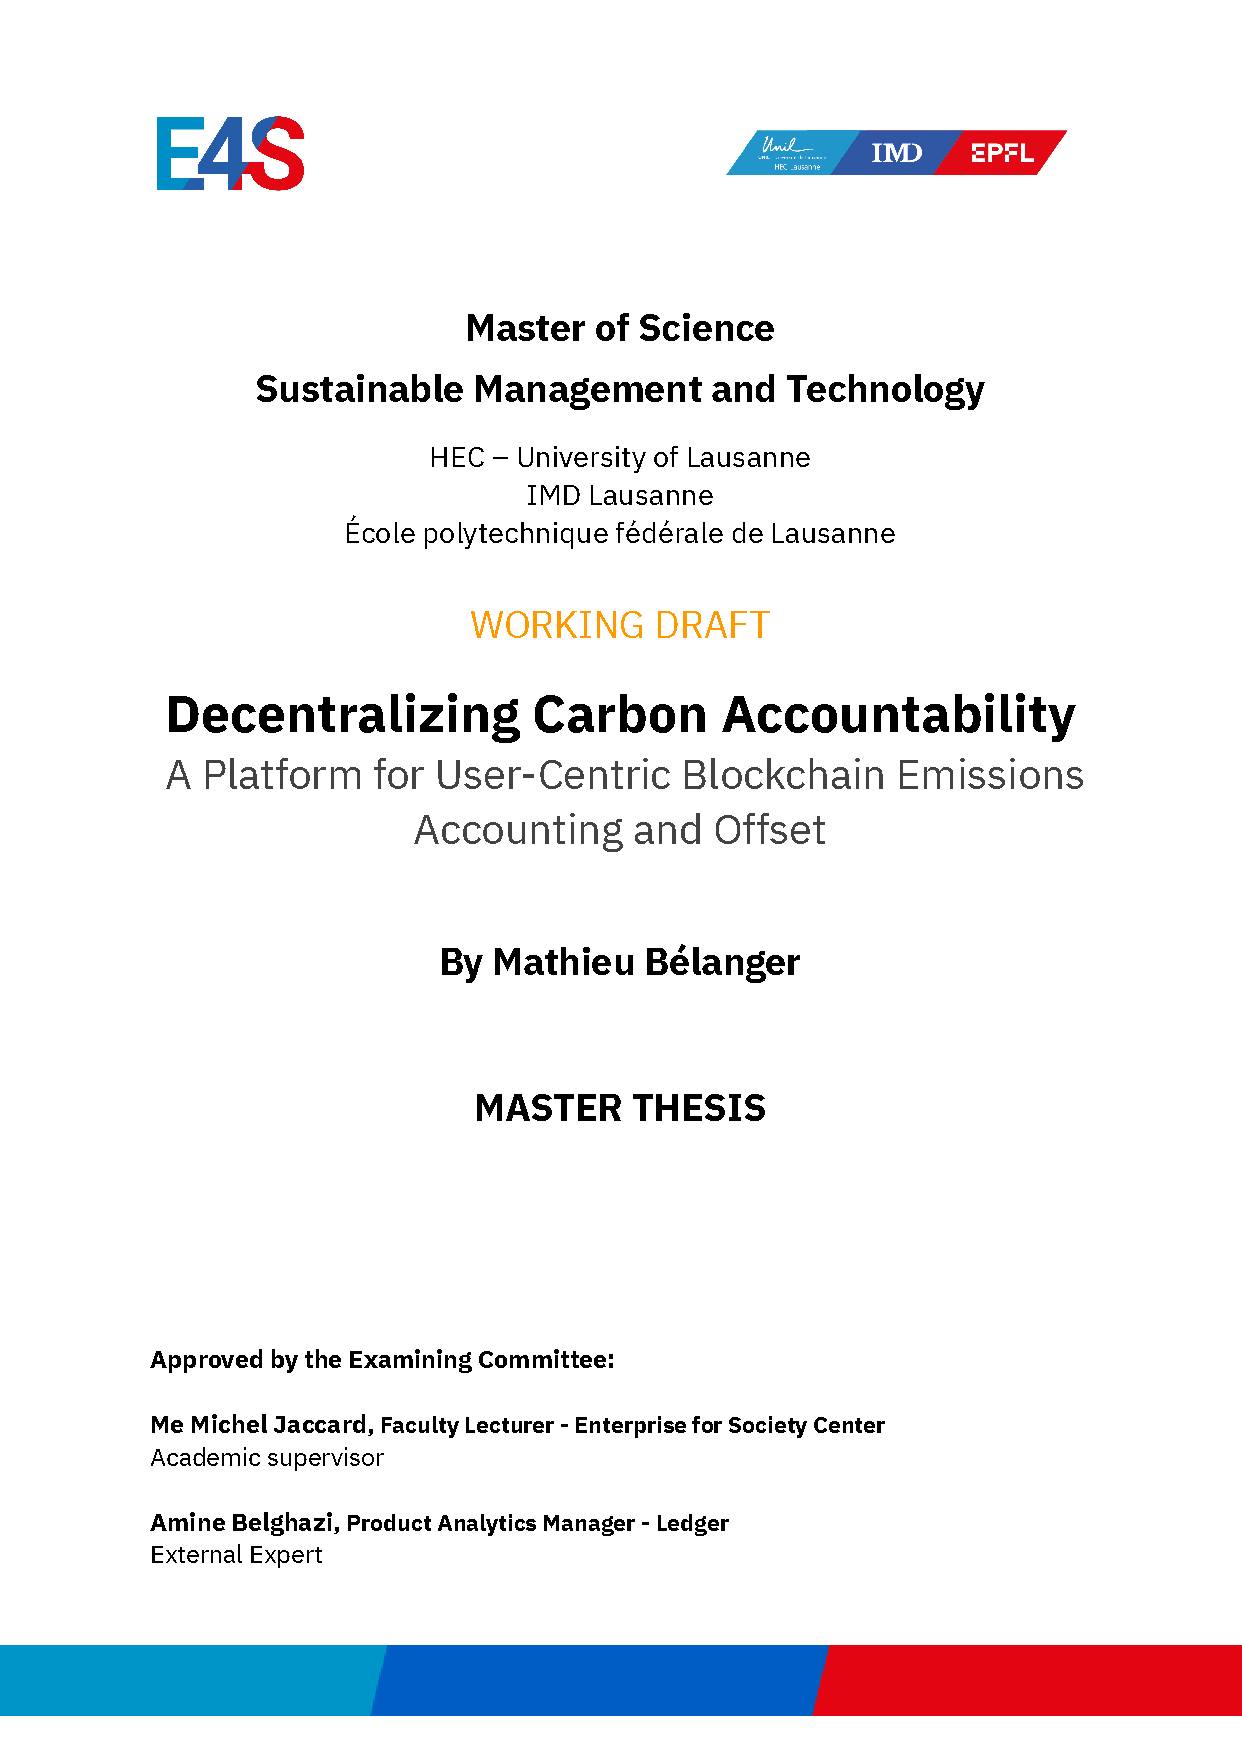
\includepdf[pages={1-2}]{cover.pdf}

% The advent of blockchain technology has raised concerns about its high energy use and carbon emissions. This is partly due to the current dominance of proof-of-work-driven Bitcoin, the first network to gain widespread adoption and media coverage. A growing research corpus has established and compared the varying environmental footprints across blockchains, resulting from different consensus mechanisms and design choices. While the recent release of the first industry blockchain ESG benchmark enables standardized comparisons between chains at an aggregate level, granular methodologies for user-level emissions accounting are still in their infancy. This thesis compares emissions attribution approaches to develop a proof-of-concept tool for user-level on-chain accounting and offsetting.

% This thesis revises attribution models designed to map the carbon footprint of blockchain at a user-responsibility level. Novel to this research is the attempt to weigh responsibility factors based on balancing the principles of proportional benefit (Beneficiary Pays Principle) and direct responsibility (Polluter Pays Principle). This approach exploits the inherent transparency of blockchain data to capture the relative value, specific to each network, that users place on different blockchain functionalities.

% Consistent with prior research, two generalizable categories of action-benefits emerge;  benefits from active transacting, and benefits from passively securing assets. The evolutions of network-specific transaction fees and market capitalization are used to weight each action-benefits in the attribution formula. All in all, it is established that hybrid attribution methods are not sufficiently accurate to be used as a standalone attribution model. However, the defined parameters can be used as separated approaches, resulting in two distinct footprint metrics. This was found to provide the most nuanced yet actionable perspective on the relative responsibility of users.

% Furthermore, a proof-of-concept tool (GreenBlocks) is built to showcase the attribution models, allowing users to estimate and offset their emissions through carbon credits. Based on the Ledger Live platform, this platform interacts seamlessly with leading blockchains and links with on-chain carbon market partners to retire offsets with maximal transparency.

% Greenblocks provides transparent and personalized insights into blockchain emissions for end-users. It enables offsets as a means for users to bear the actual costs behind the benefits they reap from using the technology. Moreover, it demonstrates the potential for on-chain data to be used as the foundation for an appropriately nuanced attribution of external costs in any system. Moving past rudimentary address metrics, more complex behaviors and benefits can be modeled, enabling the fair distribution of externalities.

\newpage
\section*{Acknowledgements}
\tableofcontents



\newpage

\section*{Structure of the Thesis}


\begin{description}
    \item [1: Introduction] \hfill \\
          A high-level overview of the topics at play. It states personal motivations that lead to the research questions and defines the thesis scope.
    \item [2: Background and Previous Work] \hfill \\
          Key concepts \& literature review covering the foundational concepts and academic work of blockchain technology, blockchain sustainability, and carbon accounting.
    \item [3. Methodology: Emission Attribution Model] \hfill \\
          From the literature review, approaches to user-level blockchain emission attribution are compared. First, a new attribution model is described. Then, the different models are implemented, and attributed emission results are compared using synthetic user data. After comparing their limitations and strengths, one approach is selected for the proof-of-concept implementation.
    \item [4. Implementation: GreenBlock Platform] \hfill \\
          Functional description and System Architecture of the proof-of-concept platform to link the selected attribution model with on-chain carbon offsetting.
    \item [5. Discussion] \hfill \\
          Results and limitations of the proof-of-concept platform. We also discuss the broader implications of user-level blockchain emission attribution for sustainability.

\end{description}

\printacronyms
\printglossary

\chapter{Introduction}

\section{Motivation}
\improvement{Compartiment in subsections to improve narrative flow}
\subsubsection*{Origins, promise, and challenges of blockchain technology}
Since the launch of Bitcoin in 2009, blockchain technology has sparked a revolution in value transfer, transparency, and decentralization \cite{nakamotoBitcoinPeertopeerElectronic2008}. However, the early meteoric rise of cryptocurrencies and underlying blockchain networks has raised critical concerns regarding their environmental sustainability. With the benefit of hindsight, we can view this period as Gartner's Peak of Inflated Expectations. Now, with notorious founders imprisoned, increasing regulatory scrutiny, and the total cryptocurrency market capitalization down
XX\% from its peak \change{cite}, the blockchain ecosystem stands at a crossroads. This is an opportunity to refocus on the core propositions of blockchain technology and ensure its long-term viability.


The dominant network, Bitcoin, which utilizes a computationally intensive proof-of-work consensus mechanism, has attracted particular scrutiny for its high energy consumption. Recent estimates indicate that the Bitcoin network alone may consume between 115 and 150 TWh annually, comparable to countries like the Netherlands \cite{devriesRevisitingBitcoinCarbon2022,neumuellerCambridgeBitcoinElectricity2021}. This growing appetite for energy competes with the just-starting energy transition, putting electrical production and distribution networks under stress. Finally, it also results in significant CO2 emissions, hardly compatible with global climate goals like the Paris Climate Accords.

\subsubsection*{Limitations of current approaches}
However, we must recognize the complexity and nuance when evaluating blockchain sustainability. Consensus protocols, design choices, and use cases vary significantly across different networks, leading to vast energy needs and emissions variability. For instance, proof-of-stake networks like Cardano and Solana promise energy savings by factors of 1000x or more compared to proof-of-work \cite{kohliAnalysisEnergyConsumption2023}. Moreover, Ethereum recently completed its highly anticipated, technically and politically complex transition from proof-of-work to proof-of-stake, demonstrating that such migrations are viable for major networks. \cite{bloombergnewsEthereumMergeYour2022} The nascent field of blockchain sustainability analysis must evolve more granular, differentiated perspectives.

Initial responses from the blockchain industry have focused on high-level aggregate comparisons and rankings between networks. For example, recent benchmarks like the \ac{CCRI} methodology provide standardized comparisons of the total lifecycle emissions across chains [5]. The institute partnered with researchers to further develop attribution methodologies in parallel to this work. The CCRI, however, adopted an opinionated approach to balancing weighing factors, and further research is needed to ensure if it is sound and if other approaches would better represent the nuances in emissions accounting and user behavior.

This poses a critical gap as blockchain technology expands into mainstream adoption. We lack diversified methodologies to attribute network-wide emissions to specific users based on their unique activity patterns and values. Such granular carbon accounting can raise awareness of individual impact and empower ethical participation.

\subsubsection*{Opportunities for user-level footprinting}

To address this, the novel approach in this thesis involves an attribution model that weighs factors like asset holdings, transactions, and computations based on their estimated importance to users on each chain. We can map emissions more accurately by considering relative user perspectives to individual entities like protocols, DAOs, or end-users. This differs from traditional carbon footprint calculators (see Figure \ref{fig:carbon_footprint_calculator}), which rely on users' self-assessment of their own behaviors in different categories of activity. This has apparent accuracy \& ergonomy issues that limit user engagement and hinder the footprint effectiveness on behavior change \cite{saloOpportunitiesLimitationsCarbon2019,mulrowStateCarbonFootprint2019}.


\begin{figure}[hbt!]
    \centering
    \centerline{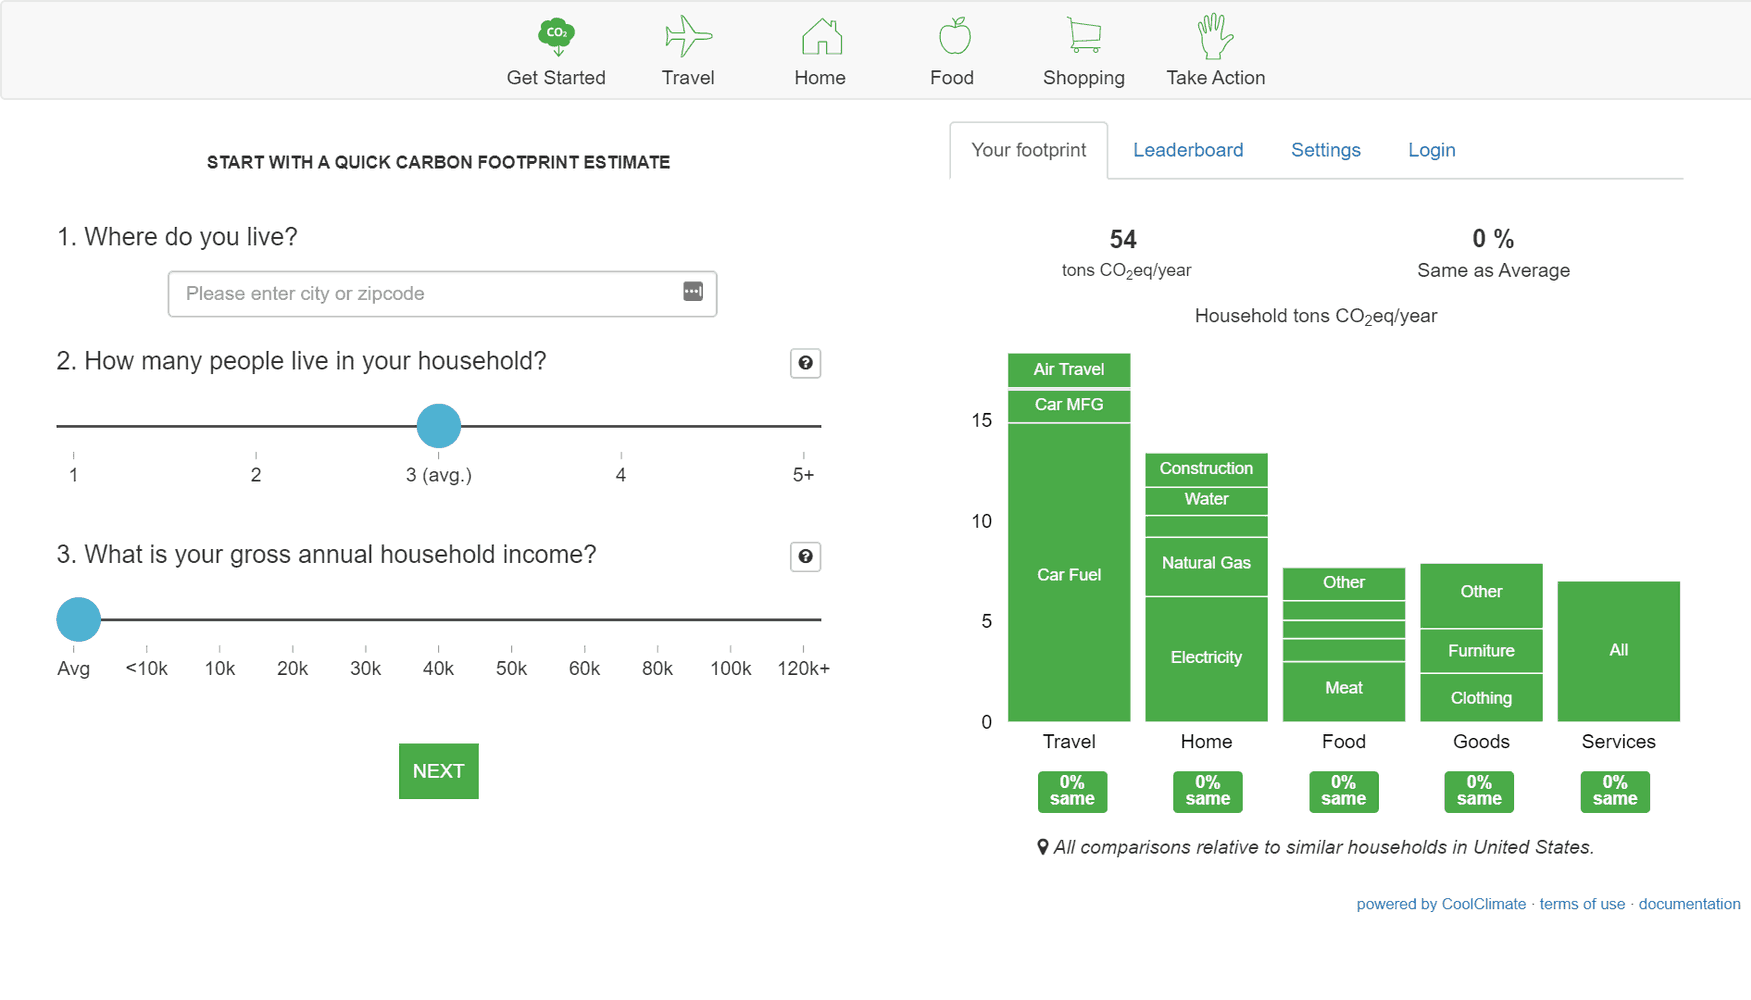
\includegraphics[scale=0.25]{figures/carbon_footprint_calculator.png}}
    \caption[YO]{Tradionnal carbon footprint calculator form - CoolClimate\footnotemark}
    \label{fig:carbon_footprint_calculator}
\end{figure}

\footnotetext{https://coolclimate.org/calculator}

Blockchain-based accounting, however, have the potential vastly improve the estimation process and reduce friction in such tool's usage. Audit of behavior history is automated and objective, not self-assessed. Here, it may first be used to provide and track basic blockchain-usage related emissions. But this proof-of-concept opens up the perspective to further use cases. Provided that more real-world behavioral and general data sources become available on-chain (with sufficient privacy features), blockchain could become a key infrastructure in modeling complex systems, fairly redistributing non direct-chain-related externalitiess. Thus, this approach unlocks new potential for transparency, responsibility, and sustainability; in the blockchain space and beyond.

As blockchain technology progresses into mainstream integration, the lack of transparency and accountability for emissions at an individual user level poses a critical gap. For example, retail investors drawn to crypto assets may be unaware of the passive environmental impacts associated with their portfolios over time. There is also an increasing offering of decentralized applications (web3) with usage beyond investing. Granular carbon accounting and attribution to individual wallets can raise awareness and enable offsetting as a means for users to take responsibility for their actions.

Moreover, this gap becomes even more complex for providers of decentralized apps or decentralized autonomous organizations (DAOs) comprising multiple smart contracts and user addresses. A DAO cannot fully assess and mitigate its overall carbon footprint without a methodology for attributing network-wide emissions based on collective usage patterns.

Therefore, the overarching problem this thesis addresses is:

"How can we design an attribution model that allocates the carbon emissions of any blockchain network to specific user entities or addresses in a transparent, accurate, and relevant manner based on their unique activity patterns?"


\section{Research Questions and Ojbectives}

To systematically address the problem of transparent and accurate carbon attribution for blockchain users and entities, this thesis pursues four key research questions:

\begin{enumerate}
    \item How can blockchain emission factors be quantified at a granular, user-centric level beyond aggregate network-wide estimates?
    \item What are appropriate metrics and weighting systems to reflect the responsibilities of diverse blockchain users based on their activities?
    \item How can we validate and demonstrate such an attribution model through a practical implementation?
    \item What are the broader implications of user-centric emissions accounting for accelerating sustainability as blockchain technology matures? \unsure{should i keep this?}
\end{enumerate}

The main objectives of this work are:

\begin{description}

    \item [Develop a User-Level Attribution Model] \hfill \\
          Develop a robust emissions attribution methodology based on usage and responsibility.
    \item [Greenblock: Practical Application] \hfill \\
          Implement and validate the model through a functional proof-of-concept application.
    \item [Promote awareness and Responsibility] \hfill \\
          of environmental impact among blockchain users.
\end{description}

\section{Scope of the thesis}

\begin{description}
    \item [Focus on Environmental Sustainability (CO2e emissions)]: Work has been done to establish blockchain footprints and impact of other axes like e-waste \cite{devriesBitcoinGrowingEwaste2021}, but the field is still developing, and data is not necessarily in a granular time-series format, essential for nuanced behavioral attribution. This thesis focuses on the most easily quantified \ac{ESG} issue, CO2e emissions, and leaves the door open for further research on other externalities (e-waste, water usage, biodiversity, social impact).
    \item [Blockchain coverage]: Only Ethereum and Bitcoin to limit data collection and aggregation complexity. As described in \ref{sec:blockchain_typology} Blockchain Typology, this covers the two main types of blockchains by functionality. This also covers the two main consensus mechanisms, \ac{PoW} and ac{PoS}, with most other post-PoW mechanisms having the same-scale environmental footprint as PoS. This is sufficient to demonstrate the model's feasibility and value. However, by Ledger's philosophy to support a wide range of blockchains, the model is designed to be extensible to other chains should the development of Greenblocks continue.
    \item [Blockchain Emissions Data sources]: This work's scope is not to critique network-level footprinting methodologies. Following the literature review, the most recognized and granular emissions data sources were identified (2), and \ac{CCRI} data was selected for the final modeling (see \ref{sec:data_sources} Data Sources). This study does not include further methodological analysis on network-level LCA and treats these data sources as ground truth. However, the model is designed to be extensible to accept combined emissions data from multiple sources should the development of Greenblocks continue.
    \item [Selection of the attribution approach]: Since the live querying of blockchain-address data was only developed during the implementation phase, this work relies on synthetic user persona data to demonstrate and compare the attribution models. The synthetic data generation, using representative statistical modeling, is detailed in \ref{sec:approach_validation} Approach to Validation.
    \item [Proof-of-concept Development]: Greenblocks, in its current form, is a prxoof-of-concept application rather than a production-ready tool. It focuses on demonstrating the potential for automating blockchain user data access. It also illustrates the user experience when reviewing its carbon footprint and the possibilities for on-chain offsetting. Refer to the Implementation section for further details on Greenblocks.
    \item [Carbon Offsets]: This thesis does not extensively review the carbon offset providers and the quality of their offering. It focuses on the technical implementation of the on-chain offsetting process and the user experience.
\end{description}


\chapter{Background and Previous Work} \label{ch:previous_work}

\todo{purpose and scope of literature review}

\section{Blockchain Technology and Its Evolution}
\unsure{This is more of a background section, but does not fit in the intro}
\subsection{Bitcoin and Proof-of-Work}
"Bitcoin: A Peer-to-Peer Electronic Cash System", the mysterious whitepaper \cite{nakamotoBitcoinPeertopeerElectronic2008}, published under the pseudonym Satoshi Nakamoto in 2008, was the first to propose a fully decentralized electronic cash system that operates based on cryptographic proof, rather than trust in a stakeholder. It introduced the concept of proof-of-work mining, a system that timestamps transactions and secures the network using computational power, negating the need for centralized control.

At its core, Bitcoin pioneered the idea of a distributed ledger - a database replicated across a decentralized network of computers; implementations of such systems are called \ac{DLT}. The Bitcoin blockchain is an immutable, transparent ledger that records the history of all transactions. Crucially, updates to the ledger are governed by a consensus mechanism that allows the participants to agree on the ledger's state without requiring a trusted third party.

While conceptual foundations for \ac{DLT} preceded Bitcoin, earlier prototypes faced limitations in achieving decentralized consensus and widespread adoption. A significant roadblock was the susceptibility to Sybil attacks, where a single entity impersonates multiple identities to exert disproportionate control.

\subsubsection{Why Proof-of-Work Enables Decentralized Consensus}

Bitcoin broke through the Sybil attack barrier by requiring proof-of-work - expending computational power - to update the ledger. This means influencing the ledger is proportional to the amount of computing work contributed. A malicious entity can no longer dominate by simply impersonating multiple identities. Additionally, Bitcoin achieves byzantine fault tolerance - the ability for a distributed system to reach consensus despite malicious nodes - by economically disincentivizing attacks on the consensus process. Proof-of-work makes attacking the system prohibitively expensive, as the computing resources would be more profitably directed at honest participation. This mechanism ensures that decision-making power stays distributed across the network nodes, paving the way for robust decentralized consensus without a central authority.

By leveraging proof-of-work to enable distributed nodes to reach consensus without a central authority, Bitcoin realized the long-standing promise of ac{DLT}. For the first time, a decentralized peer-to-peer network could self-govern through an incentives system, building an open consensus mechanism resistant to takeover. This solution enabled the emergence of Bitcoin as the first decentralized digital currency to gain real-world traction.

\subsection{Ethereum and Smart Contracts}

The Ethereum whitepaper\cite{buterinEthereumNextgenerationSmart}, published by Vitalik Buterin in 2013, proposed enhancements to Bitcoin's core concepts, allowing arbitrary computer code to be validated and executed by the network. It introduced smart contracts, which are executable programs hosted on the network that can encode complex logic and state, going beyond Bitcoin's simple cash transfer function. From simple use cases like access and withdrawal rules for a multi-owner bank account to trustless lending platforms to complex interactions between contracts and real-world data-delivering insurance instruments, the possibilities kept growing as building blocks get developed, and data from the outside world are bridged on-chain\footnote{https://chain.link}. These decentralized applications (dapps) leverage Ethereum's distributed ledger features.

The \ac{DLT} features of such apps have also been leveraged in the sustainability space, with recent successful implementation of renewable energy credit trading and verification (Danish Condordium Blockchain\footnote{https://concordium.com/all-news/the-concordium-blockchain-contributes-to-danish-transmission-energinets-new-green-energy-certificate-platform}), or forward carbon credits leveraging citizen science and satellite data (Solid World\footnote{https://www.solid.world}). Ethereum also improved upon Bitcoin's design, with ongoing changes implementing transaction-throughput scaling solutions. While Bitcoin demonstrated \ac{DLT}s currency applications, Ethereum expanded the potential of blockchains to diverse sharing economies, financial services, identity systems, and beyond.

\subsubsection{Building the chain while flying it}
As it was first conceived (V. Buterin's \textit{White} paper) \cite{buterinEthereumNextgenerationSmart} and implemented (G. Woods \textit{Yellow} paper)\cite{woodEthereumSecuredDecentralised2023}, ethereum launched using a bitcoin-PoW-derived consensus mechanism. This went against initial plans to adopt a more energy-efficient one. Game-theory researchers' interest had sparked after bitcoin's rise, and few novel alternative sybil/byzantine resilient consensus mechanisms were being developed. However, at the time of implementation, with pressure from investors to launch the network, the Ethereum Foundation fell back to using PoW as it was the most mature and tested mechanism. This severely affected the historical network's electrical consumption; the planned transition lasted much longer than expected (more in section \ref{sec:ethereum_transition}).

With the first live-operating network able to make the switch and ecological considerations growing, many hoped Bitcoin would soon follow.  Nevertheless, Bitcoin miners have everything to lose from the transition, and failing to put a majority of stakeholders on board would rip the ecosystem into multiple separate networks, signaling the end of Bitcoin supremacy. This politically hard-to-navigate situation, added to skepticism towards PoS tradeoffs concerning the blockchain trilemma (see Figure \ref{fig:blockchain_trilemma}), still makes it a difficult buy for Bitcoin's change-reluctant community. More on the environmental aspect of this transition in section \ref{sec:ethereum_transition}.

\subsection{Miner Incentives in \ac{PoW}}

An important notion to understand the dynamics of blockchains is the incentive equilibrium that drives miners to participate in the consensus process. In the bitcoin \ac{PoW} case, two mechanisms are used: block reward (newly minted coins attributed to the winner for each block added to the chain) and transaction priority fees. As specified in Nakamoto's paper \cite{nakamotoBitcoinPeertopeerElectronic2008}, block rewards will keep decreasing over time until reaching zero, at which point transaction fees will be the only incentive for miners to participate in the consensus process. The projected long-term impact of this incentivization policy is described in \cite{easleyMiningMarketsEvolution2019}. An essential projection is that the decision to increase the block size, a tradeoff between security and transaction throughput, historically rejected by the community, will eventually be championed by miners as transaction fees become the only incentive for mining. This shift in the incentive structure makes the network security gradually more dependent on users' willingness and capacity to pay for transaction fees.

\begin{figure}[hbt!]
    \centering
    \centerline{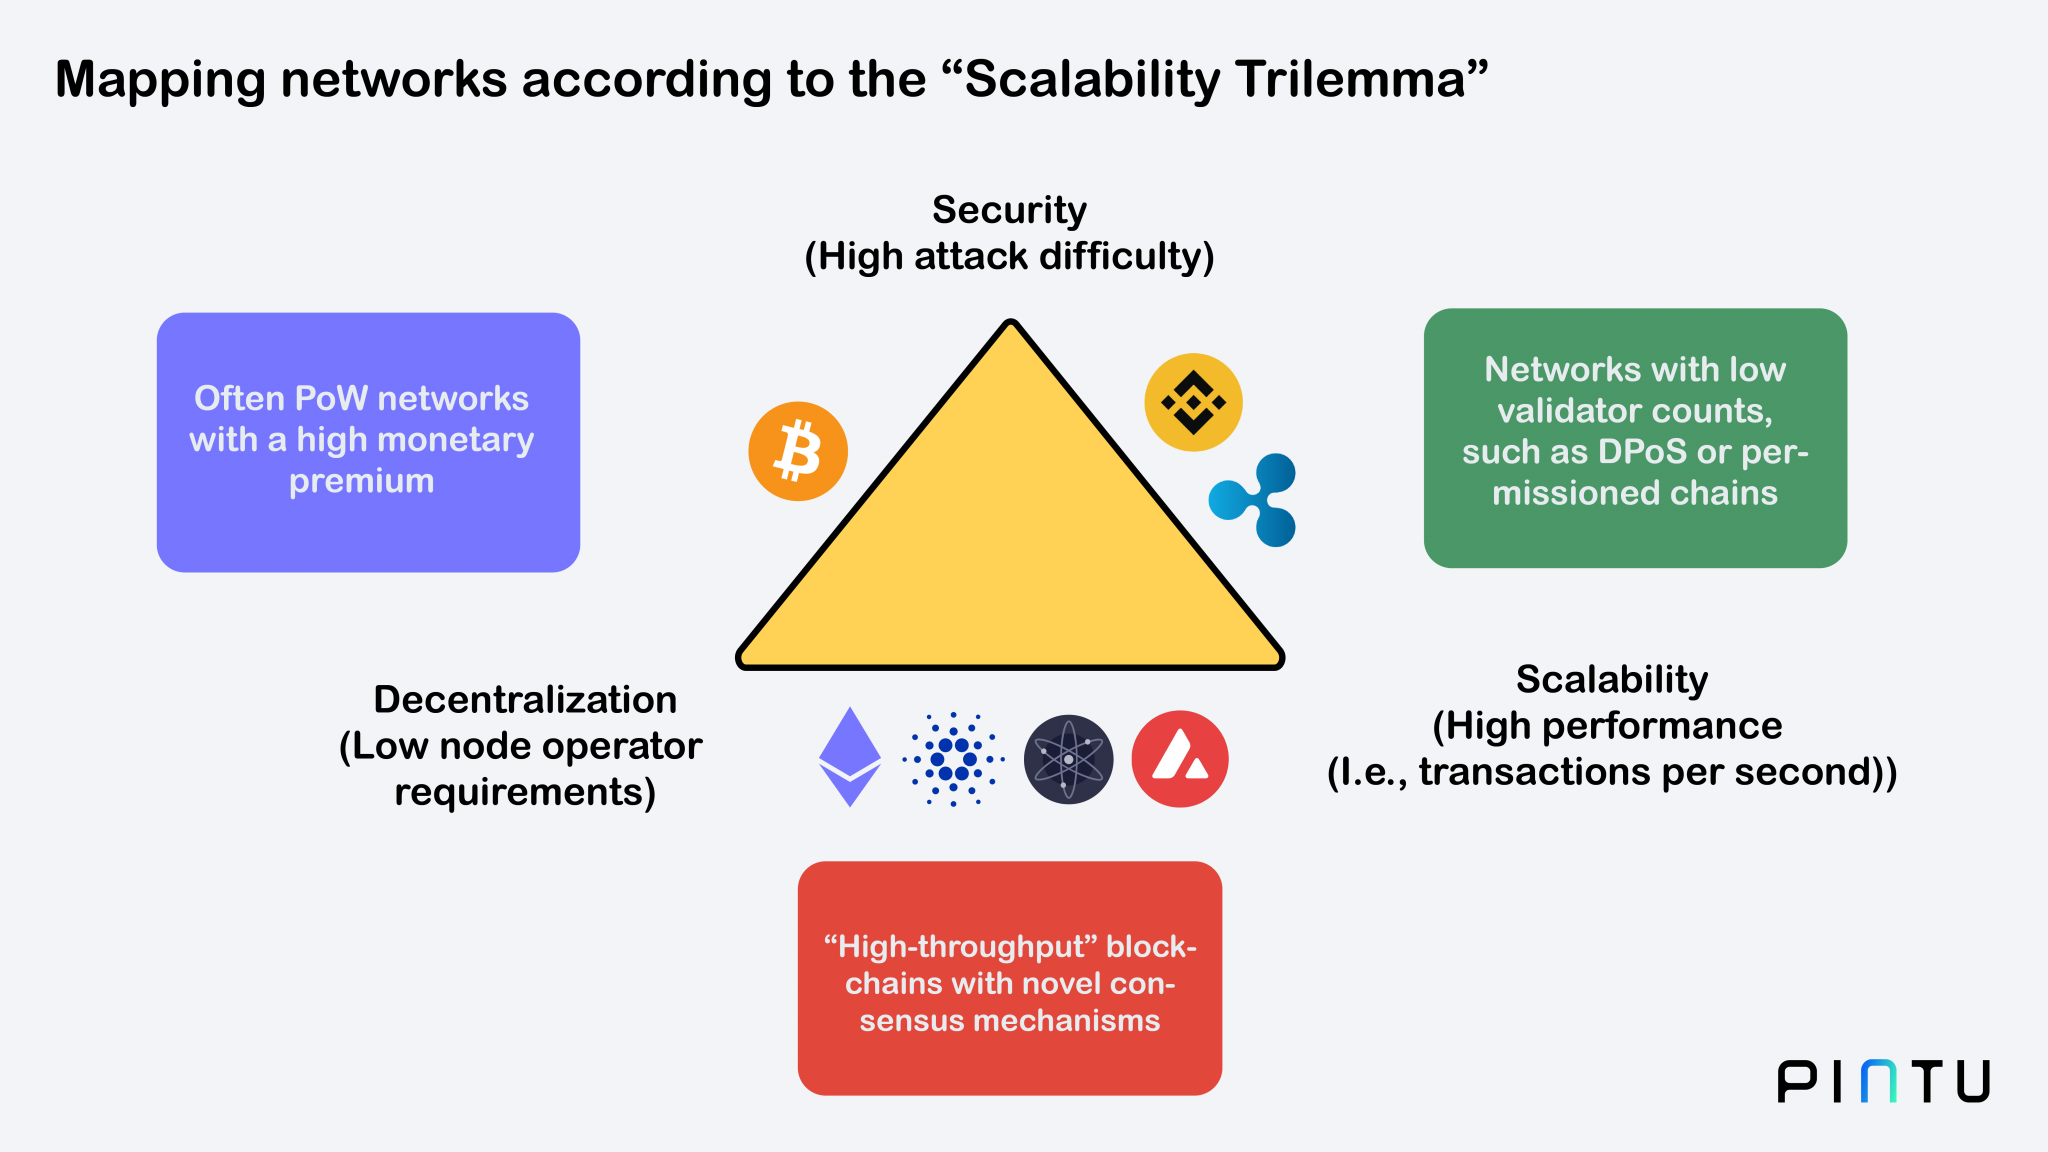
\includegraphics[scale=0.23]{figures/blockchain_trilemma.png}}
    \caption[YO]{The Blockchain Features Trillema}
    \label{fig:blockchain_trilemma}
\end{figure}


\section{Environmental Impact of Blockchains}
\subsection{Bitcoin and Proof-of-Work}
The environmental impact of Bitcoin, driven by its proof-of-work consensus mechanism, has become an essential focus in research and public discussion. The main concern is Bitcoin's energy-intensive mining process and associated carbon emissions. As research has evolved, a nuanced understanding of Bitcoin's environmental footprint requires examining multiple factors, combining economic modeling and empirical data analysis. Estimates can adopt two different approaches: top-down or bottom-up. Top-down approaches infer energy (and emissions) use from the evolving valuation of mined tokens, applying hypothesis on aggregate miners' economics and behavior. Bottom-up approaches, on the other hand, are slightly more complex. They use empirical data on available hardware and transparent network hash rate data (the evolving mining difficulty factor specific to each chain) to work upwards to overall energy use and emissions. The following sections review the main findings from both approaches.

\textbf{Bitcoin's Energy Consumption}

De Vries (2018) \cite{devriesBitcoinGrowingEnergy2018} shed light on Bitcoin mining's vast energy demands, estimating the network could consume over 73 TWh/year at peak performance, approaching entire countries' consumption. This stemmed from the immense computational power needed for mining, with energy expenditures of 300-900 kWh per transaction. De Vries' analysis used economic models, suggesting miners operate up to where electricity costs dominate marginal costs. De Vries used a top-down approach.

Stoll et al. (2019) \cite{stollCarbonFootprintBitcoin2019} refined these estimates using a techno-economic approach, still considered top-down. They diverged from De Vries in deriving hardware efficiency data from mining manufacturer IPOs and using IP geolocation for localized emission factors. Their findings showed 45.8 TWh consumption in 2018, substantial but below De Vries' projection. Incorporating IP distribution scenarios offered valuable localization insights into Bitcoin's energy sources.

\textbf{Beyond Energy: Environmental Externalities}

While energy is the primary focus, De Vries (2021) \cite{devriesBitcoinGrowingEwaste2021} highlighted another issue: e-waste. Mining hardware obsolescence contributes over 30.7 metric kilotons/year of e-waste, underscoring Bitcoin's multifaceted environmental challenges beyond energy. De Vries' lifecycle analysis methodology offered more rigorous e-waste estimates than previous energy-focused models.

\textbf{Impacts of Regulatory Shifts}


Bitcoin's dynamic landscape, influenced by regulation, also affects its environmental impact. De Vries (2022)\cite{devriesRevisitingBitcoinCarbon2022}  revisited Bitcoin's carbon footprint after China's 2021 mining crackdown. This led renewable energy's share in mining to drop from 42\% to 25\% as miners relocated to Kazakhstan and the US. Such shifts demonstrate Bitcoin's unstable regulatory landscape and the dramatic impact it can have on environmental performance.

\textbf{Live Emission Monitoring}

The Cambridge Bitcoin Electricity Consumption Index \cite{neumuellerCambridgeBitcoinElectricity2021} and accompanying Greenhouse Emissions Index
exemplify cutting-edge emission monitoring, continually tracking Bitcoin's emissions using real-time, localized data and daily emission factors. This robust bottom-up approach captures the dynamics of cryptocurrency mining emissions and has been corroborated by other methodologies, including different bottom-up estimates \cite{mcdonaldEthereumEmissionsBottomup2022}.

\section{Ethereum, the Succesful Case for a Transition to Proof-of-stake \label{sec:ethereum_transition}}

Ethereum's recent shift from the energy-intensive "proof-of-work" consensus mechanism to the more sustainable "proof-of-stake" in September 2022 has transformed the cryptocurrency landscape. This transition, known as "the Merge", was long delayed due to the technical and political complexities putting in jeopardy a successful transition\cite{bloombergnewsEthereumMergeYour2022}. Now achieved, it positions Ethereum as a leader in blockchain sustainability\footnote{https://ccdata.io/research/esg-rankings} and sets a precedent for other major cryptocurrencies to consider transition. With Ethereum's move expected to reduce its carbon footprint drastically, the focus is turning to Bitcoin's potential trajectory. While the two platforms serve different primary functions, Ethereum's successful transition raises the question: Could Bitcoin be next to adopt a greener consensus mechanism?


\textbf{Ethereum's Energy Use (PoW)}

McDonald (2022)\cite{mcdonaldEthereumEmissionsBottomup2022} tackled Ethereum's energy footprint through a meticulous bottom-up approach. By compiling data on network hashrates, hardware efficiencies, and even data center overheads, McDonald thoroughly modeled Ethereum's consumption at ~60 TWh over seven years. Aligning with top-down estimates, this empirically grounded, best-practice approach highlighted the need for more sustainable consensus mechanisms.

\textbf{Exploring PoS' Potential}

Exploring PoS as an energy-efficient PoW alternative has gained momentum. Platt et al. (2021)\cite{plattEnergyFootprintBlockchain2021} analyzed PoS chains' energy needs, pioneering a model weighing factors like validator counts and node power. Findings were promising: PoS chains consumed far less energy than PoW counterparts, with some even outperforming centralized systems like VisaNet.

Ibanez (2023) built on this, validating the model's core findings while highlighting nuances in consumption across PoS systems. Crucially, their research emphasized PoS systems' relative efficiency compared to heavyweights like Bitcoin.

\textbf{Ethereum's PoS Transition: A Case Study}

Ethereum's 2022 merge to PoS marked a sustainability milestone. De Vries (2022)\cite{devriesCryptocurrenciesRoadSustainability2022} examined this transition. The post-merge energy use reduction has been impresive - nearly 99.95\%, equivalent to a country like New Zealand's electricity. This number has also been corroborated by Cambridge's blockchain index team, reporting a reduction going up to 99.99\%\cite{CambridgeEthereumElectricity}. While challenges around e-waste and wealth concentration risks remain, Ethereum's move sets a precedent, demonstrating blockchains can scale sustainably.

\section{Carbon Accounting - User-Level Emissions Attribution}

\subsection{The Polluter \& Beneficiary Pays Principles}

{\large{TODO}}\todo{TODO}

\subsection{Traditional Individual Carbon Footprint \label{se:traditional_footprint}}

As seen in figure \ref{fig:carbon_footprint_calculator}, traditional footprint calculators usually rely on users' self-assessment of different emissions categories. This has obvious limitations regarding ergonomy and induces friction in the footprinting process. Users must fill out a questionnaire to get their number, with the accuracy proportional to its length. Moreover, it is error prone as users over/underestimate or misremember previous behaviors. The friction in filling out the form makes it unrealistic to use it regularly and does not allow users to track their progress. This is a major limitation of behavior change. \todo{cite}. Blockchain data transparency and attribution make it possible to automate the process and vastly increase accuracy as it applies the same rules to everyone.

\subsubsection{Carbon Offsets - The Voluntary Carbon Market}
\subsubsection{Traditional Offsets - Limitations}


Limited User engagement towards footprint calculators, tedious process, and error-prone

\todo{This user experience will be improved with blockchain data transparency and attribution. Link with further use sustainability use cases. Blockchain-based footprints make it possible to automate the process and vastly increase accuracy as it is no longer a self-assessment. Cite issues of carbon footprint calculator accuracy because of self-assessment.}

\subsection{On-Chain Accounting \label{se:onchain-accounting}}

Amid rising institutional concerns about cryptocurrencies' environmental impact, the Crypto Carbon Ratings Institute's (2023)\ revised white paper provides a timely, nuanced perspective. By thoroughly examining the carbon footprints of both PoW and PoS networks, the paper introduced a \textit{hybrid allocation} approach for emissions accounting in its most recent version. This methodology recognizes that network energy use stems from both holdings and transactions.

It expands on previous work by De Vries (2021) \cite{devriesTrueCostsDigital2021}, early attempts to address balance emissions attribution methodology for bitcoin. The CCRI's methodology now covers a wide range of networks, differentiating between PoS and PoW in the attribution strategy. Specifically, they use a combination of the Cambridge Index \cite{neumuellerCambridgeBitcoinElectricity2021}, de Vries "Revisiting Btcoin's carbon footprint" \cite{devriesRevisitingBitcoinCarbon2022} and Gallersdörfer's work \cite{gallersdorferEnergyConsumptionCryptocurrencies2020} for PoW chains (Bitcoin, ETH PoW in our case). For PoS networks (ETH PoS in our case), the methodology is reported in their own \textit{ETH Merge Report}\cite{ETHMergeReport}, it expands on the work of Platt et al. (2021)\cite{plattEnergyFootprintBlockchain2021} and Ibanez et al. (2023)\cite{ibanezEnergyConsumptionProofofStake2023}.

\textbf{The Hybrid Emissions Allocation Approach}

The "hybrid allocation" approach is a significant contribution, merging holding-based and transaction-based emissions accounting for a comprehensive view of blockchains' environmental impact. For PoW chains, the relationship between block rewards and transaction fees is used to weigh both variables in the attribution formula. According to the authors, this proportion "determines the distribution of the electricity consumption between holding and transactions executed." For PoS chains, the marginal power demand resulting from processing transactions is used as a share of total demand Real-world data sources like CBECI and their own CCRI-API back this methodology.


\textbf{Bringing Offsets On-Chain - Opportunities}






\section{Research Gap}

\subsection{Identifying a research gap}

user-level attribution research is scarce

we should analyze CCRIs hybrid allocation and compare it to other approaches as its weigth factor is the result of a subjective decision



While aligning with the CCRI's recent approach to hybrid attribution, this research introduces the "Beneficiary Pays Principle" to weigh emissions responsibility based on users' perceived value from blockchain functions. This user-centric approach provides a differentiated perspective to the paper's focus on block rewards and fees.

Moreover, the CCRI paper lacks a practical implementation of its methodology and beyond user-example results. This thesis addresses this gap by building a proof-of-concept application to demonstrate the attribution model's feasibility and value.

    {\large{TO CONTINUE}} \todo{TO CONTINUE}

\chapter{Methodology: User-Level Emissions Attribution Model}
\section{Overview \label{se:methodology_overview}}

\todo{Find where to include steps of the work. Interviews and data collection}

This chapter maps and compares the possible approaches ensuring display of legitimate, nuanced and actionnable user-level footprints in the PoC.

First, a typology of blockchains is proposed to enable the proper selection of metrics relevant to networks' distinctive characteristics. Then it is shown that using stakeholders' active behavior (sending transactions) as the sole attribution parameter does not lead to a fair share of responsibility for the network's environmental externalities. This leads to the definition of a second parameter based on passive behavior (holding assets). To combine the parameters in a single footprint, we introduce a novel methodology to attribute network emissions to addresses based on proportional benefits gained by users.

This methodology is underpinned by ethical and ecological theories suggesting externalities be allocated based on the proportional benefits stakeholders gain from presence in a system. Historical trends in network metrics like fees and market value provide proper signals into evolving blockchain utility dynamics and user perceptions of value.

Finally, the results section compares the proposed methodologies using synthetic user data. Moreover, experts interviews from members of the industry and academia have been conducted to help inform the analaysis. This work tries to establish a nuanced and fair approach to emissions attribution. This approach should be aligned with the real-world value stakeholders obtain from blockchain networks, leaving them actionable steps to improve. The following sections detail this approach and rationale.

\section{Background - Emission attribution considerations}

\subsection{Blockchain Typology \label{sec:blockchain_typology}}
Blockchains can be categorized into two main types based on their primary function and underlying mechanics:
\improvement{This separation is also justified by the polluter and beneficiary pays framework. The limited resource (block space) is shared differently for Bitcoin and Ethereum}

\begin{description}
    \item[\ac{VTC}] Chains that focus on transferring assets between addresses (e.g. Bitcoin and derived). VTCs are focused primarily on enabling value transfers through native cryptocurrency tokens. These chains do not typically support complex smart contract functionality like GPCs or make similar functionalities unergonomic to implement. The key operational metric for VTCs is the transaction throughput, constrained by block sizes and block intervals.

    \item[\ac{GPC}] Chains that allow the deployment of smart contracts and decentralized applications (dApps) in addition to value transfer (e.g. Ethereum, Cardano, Solana). On these networks, transactions and computations are quantified using a metric called gas\footnote{See: https://ethereum.org/en/developers/docs/gas/}. This concept was introduced by Vitalik Buterin in Ethereum's initial whitepaper \cite{buterinEthereumNextgenerationSmart} as a means to disincentivize computationally intensive smart contracts that could clog the network. Gas puts a cost on network utilization for activities like executing code, storing data, or transferring tokens based on their computation complexity. This makes it more costly to interact with complex applications and prevents situations that would halt the network like an infinite loop in a smart contract.
\end{description}

Due to these fundamental differences, GPCs and VTCs require distinct approaches for carbon accounting. On VTCs, the limited block space is the bottleneck for transactions. Hence, users conducting more transactions take up a greater share of blockspace and have higher responsibility for the chain's emissions. On GPCs, gas expenditure more accurately reflects utilization and impact on the network's computation and storage load. Users spending more gas have a greater share of responsibility by consuming more of the network's resources and throughput capacity. This distinction follows both the \textit{Polluter Pays} and \textit{Beneficiary Pays} principles as direct responsibility and benefits are aligned.

Existing studies have estimated blockchain emissions using aggregate network energy use or miner rewards \cite{devriesCryptocurrenciesRoadSustainability2022,devriesRevisitingBitcoinCarbon2022,neumuellerCambridgeBitcoinElectricity2021,mcdonaldEthereumEmissionsBottomup2022}. However, these top-down approaches fail to capture user behavior and responsibility. Our methodology addresses this limitation through a transparent attribution model tailored to GPCs and VTCs using usage factors like gas and transactions. The following sections detail this framework.

\subsection{Attribution framework}
\improvement{To review!! Add share infrastructure metaphor. Introduce polluter/benef pays from the litt review.}
The Need for Proportional Benefit Attribution
Carbon emissions from blockchain operations should be tied to direct causative actions (polluter pays principle) and the benefits derived from these actions (beneficiary pays principle). The synthesis of the polluter pays and beneficiary pays principles results in a more nuanced understanding of emission responsibility.

    {\large{YOOOO}}

This thesis revises attribution models designed to map the carbon footprint of blockchain at a user-responsibility level. Novel to this research is the attempt to weigh responsibility factors based on balancing the principles of proportional benefit (Beneficiary Pays Principle) and direct responsibility (Polluter Pays Principle). This approach exploits the inherent transparency of blockchain data to capture the relative value, specific to each network, that users place on different blockchain functionalities.

\subsubsection*{Transactional Activities}

Direct Actions and Associated Benefits
Signing transactions or spending gas actively utilizes block space, a limited resource. This results in emissions and is a direct reflection of users seeking to derive transactional benefits from the blockchain. By engaging in these activities, users contribute to emissions and benefit from the network's utility.

\subsubsection*{Beyond Transactions: Passive Utility and Continuous Benefit}
While active behaviors like transactions and gas spending are evident, users gain a passive benefit simply by holding assets on the network. This benefit accrues continuously over time and is inherently dependent on the active behaviors of others. Passive holders benefit from the blockchain's ability to secure value, beyond the direct actions of signing transactions or spending gas. This implies an added layer of responsibility that isn't captured by looking at transactions alone.

\subsubsection*{Balancing the Attribution: Weighing Active and Passive Benefits}
With two distinct parameters (active transactions/gas spending and passive holding of value), there's a need to determine their respective weights in the attribution formula. The conjunction of the polluter pays and beneficiary pays principles demands understanding the relative utility of active and passive benefits to users.

\subsubsection*{Deriving Weights Factors: The Role of Transaction Fees and Market Capitalization}
Historical trends of transaction fees and market capitalization serve as proxies to establish the relative importance of active versus passive benefits. These indicators reflect user-perceived utility and significance of both benefits over time. Transaction fees offer insights into the value users associate with active transactional capabilities, while market cap reflects the trust and perceived security in the network's ability to hold value. These can be used to derive dynamic weights for the two parameters in the emission attribution formula.



\subsubsection*{On Including Passive Holdings as a Responsibility parameter}
A key differentiator is the inclusion of historical balance as a responsibility factor. Traditionally, emissions accounting ties responsibility to direct actions like executing transactions or computations. \improvement{Add metaphor of traditional infrastructure. Roads and km usage vs. passive benefit of the road proximity} However, in blockchains, holding assets passively (function of preserving/securing value) also necessitates ongoing mining and transaction fees paid by transacting users to preserve liquidity and value.

\improvement{Put justifications in list form to emphasize each point}

Specifically, continuous mining activity and block creation are critical to maintaining an active market and allow holders to liquidate assets. In the bitcoin case, miner rewards are increasingly coming from transaction fees only, as block rewards shrink over time in a process called \textit{halving} \footnote{https://www.investopedia.com/bitcoin-halving-4843769} To that effect, miner activity is increasingly reliant on user's transaction fees. Higher fees increase miner rewards and impact profitability, resulting in an arms race in mining (compute) capacity. This is a key factor in the network's security and makes Bitcoin holders' asset security dependent on the active transactional behavior of other users \cite{easleyMiningMarketsEvolution2019}. In the Ethereum case, since the switch to proof-of-stake consensus, reward attribution is more complex but still reliant on transaction fees, varying with the demand in block space. The demand in blockspace combines the number of transactions and their computational complexity, measured in gas.

TO BLEND
Holding assets does not induce direct additional emissions, but benefits from these functional units are dependent and proportional to continuous transactions signed by other users. With fewer new transactions, lower fees are being paid to incentivize miners' work, thus lowering chain security and reducing the cost of an attack. With fewer transactions being signed and lower incentives, miners' profitability is diminished.  In the mid-term, this will result in fewer and lower investments in mining computing power, reducing the cost of an attack and the overall network security. The holder's benefit (securing value) is also derived from the inflow-outflow of tokens to centralized exchanges where they can be traded against fiat currencies, increasing the liquid aspect of the token and actualizing its value. \todo{blend this in the section}

Therefore, despite no active behavior, holding blockchain assets creates a latent demand for emissions-intensive mining. Considering this relationship, the attribution model argues for allocating part of emission responsibility to asset holders or, more generally, to how intensively a user uses the blockchain function of securing value.

\section{Model Components}

Building on the previous overview, this section details the specific components of the emission attribution model.

\subsection{Historical Blockchain Emissions Data}
\todo{expand, explain LCA amortized emissions}
The emission rate \(E(\tau)\) represents the overall amount of tCO2-equivalent emissions generated by a blockchain at time $\tau$. This is chain-specific, with data aggregated from existing studies \cite{neumuellerCambridgeBitcoinElectricity2021,stollCarbonFootprintBitcoin2019}.

\begin{equation}
    E(\tau) = \text{Emission rate of chain $s$ at time $\tau$}
    \label{eq:emission_rate}
\end{equation}

\todo{Detail combination of papers and dataset access}

\subsection{User Attribution Parameters}

The attribution share ($S$) for an address owned by a user is proportional to the measurement of two categories of behavior-benefits. Interactive behavior ($I$) is directly responsible for a share of emissions and reaping direct benefits from the network interaction, and Passive behavior ($P$) indirectly accrues benefits from the network's ongoing operation. Three possibilities are then considered for the attribution share, expressed in the following equations:

\begin{align}
     & S \propto (P \wedge I) \\
     & S \propto P            \\
     & S \propto I
    \label{eq:attribution_share}
\end{align}

Hybrid Attribution (equation 3.2) considers a weighted combination of interactive and passive behavior, resulting in a single metric. Additionally, we also consider the two parameters separately, as they provide distinct insights into user behavior and responsibility. This gives the \textbf{Passive or Balance-based Attribution} and \textbf{Interactive or Transaction-based Attribution} (equations 3.3 and 3.4) models.

Interactive behavior is measured by the share of network resources (block space) allocated to the user's address for his interactions during a period. For \ac{VTC}s, this is reported by the number of signed transactions; for \ac{GPC}s, it is the sum of gas spent in signed transactions. Passive behavior is measured by the share of the total value secured by the network owned by the user's address.

The three factors are, for an address on a given chain and at period $\tau$:

\begin{description}[leftmargin=!, labelwidth=\widthof{\bfseries Passive Behavior}]

    \item[Interactive Behavior $(I)$] \hfill
        \begin{itemize}[labelwidth=4cm, align=left, labelsep=0pt]
            \item[\( T(\tau) = \frac{T_{addr}(\tau)}{T_{\text{total}}(\tau)} \)]
                Number of transactions signed by the address as a percentage of total transactions (for VTCs).

            \item[\(G(\tau) = \frac{G_{addr}(\tau)}{G_{\text{total}}(\tau)} \)]
                Gas spent by the address as a percentage of total gas in blocks (for GPCs).
        \end{itemize}

    \item[Passive Behavior $(P)$] \hfil
        \begin{itemize}[labelwidth=4cm, align=left, labelsep=0pt]
            \item[\(B(\tau) = \frac{B_addr(\tau)}{B_{\text{total}}(\tau)} \)]
                Average address Balance as a percentage of total token supply.
        \end{itemize}

\end{description}
\parsep 5pt
Thus, from equation \eqref{eq:attribution_share}, we have the chain-specific emission attribution share for an address at period $\tau$:


\begin{equation}
    S(\tau) \propto \left[B(\tau) + \begin{cases}
            T(\tau) & \text{for VTC} \\
            G(\tau) & \text{for GPC}
        \end{cases}\right]
    \label{eq:attribution_share_chain_type}
\end{equation}

\subsection{Weighting factors (Hybrid Attribution) \label{se:weighting_factors}}

Introducing a second attribution parameter for the hybrid attribution method raises the question of how to weigh the two factors. The attribution share is proportional to the sum of the two factors, but the relative importance of each is not clear. To address this, we derive weights for each attribution parameter based on the principle of proportional benefits. Adding the weigh factors to each parameter in equation \ref{eq:attribution_share} we now have:

\begin{align}
     & S(\tau) = (\alpha \cdot P + \beta \cdot I)                                  \\
     & S(\tau) = \left[\alpha \cdot B(\tau) + \beta \cdot \begin{cases}
                                                                  T(\tau) & \text{for VTC} \\
                                                                  G(\tau) & \text{for GPC}
                                                              \end{cases}\right]
    \label{eq:attribution_factors}
\end{align}



Blockchain networks and user behaviors evolve over time. As such, users' relative importance on transactional versus asset-holding utility can shift. The factors $\alpha$ and $\beta$ are estimated by analyzing historical trends in transaction fees and market capitalization to account for these dynamics. This is done for each supported chain.

\begin{description}
    \item[Transaction Fees $F$]: As users invest more in transaction fees, it's an indicator that they're deriving value from the active functionalities of the blockchain. A rise in these fees underscores a user trend prioritizing transactional abilities. For \ac{VTC}s, this is the average transaction fee per block; for \ac{GPC}s, it is the average gas price per block.
    \item[Market capitalization $M$]: Indicates user trust in the blockchain as a secure store of value. Growth in market cap highlights increasing passive utility perceived by users.
\end{description}

\subsubsection{Quantifying Shifts in User Priorities}

By tracking the relative changes in transaction fees and market cap over time, the model adapts to users' shifting priorities. First, the relative change for each metric is calculated across the emission attribution interval, limited by the granularity of historical data available.

\begin{align}
    \bar{\Delta F} & = \frac{1}{N}\sum_{i=1}^{N}\frac{F(\tau_i) - F(\tau_{i-1})}{F(\tau_{i-1})} \\
    \bar{\Delta M} & = \frac{1}{N}\sum_{i=1}^{N}\frac{M(\tau_i) - M(\tau_{i-1})}{M(\tau_{i-1})}
\end{align}

\improvement{Maybe add a figure to illustrate the concept}


Where \( N \) represents the number of time intervals.

The ratio of these changes is the relative importance of transactional benefits to passive benefits. This is the basis for the attribution weights.

\begin{equation} \label{eq:weights_ratio}
    \bar{R} = \frac{\bar{\Delta F}}{\bar{\Delta M}}
\end{equation}

The relationship ratio $\bar{R}$ represents the relative importance between transaction fees and market capitalization. To convert this into proportional weights summing to 1, the transformation of equation \eqref{eq:alpha_weight} is used.

\begin{equation} \label{eq:alpha_weight}
    \alpha = \frac{\bar{R}}{1 + \bar{R}}
\end{equation}

Subsequently, \( \beta \) is:
\begin{equation} \label{eq:beta_weight}
    \beta = 1 - \alpha
\end{equation}


\subsection{Attributed Emissions \label{se:attributed_emissions}}

Multiplying chain emission rate \eqref{eq:emission_rate} with the sum of attribution parameters \eqref{eq:attribution_share_chain_type} and corresponding weights \eqref{eq:alpha_weight} and \eqref{eq:beta_weight}, we get the CO2e emissions \(A(\tau)\) attributed to an address on a given blockchain for the period $\tau$ general form:

\textbf{Hybrid Attribution}
\begin{align}
    A(\tau) = E(\tau) \times \left[\beta \cdot B(\tau) + \alpha \cdot \begin{cases}
                                                                              T(\tau) & \text{for VTCs} \\
                                                                              G(\tau) & \text{for GPCs}
                                                                          \end{cases}\right]
\end{align}

\textbf{Transaction-based Attribution}
\begin{align}
    A(\tau) = E(\tau) \times \begin{cases}
                                 T(\tau) & \text{for VTCs} \\
                                 G(\tau) & \text{for GPCs}
                             \end{cases}
\end{align}

\textbf{Balance-based Attribution}
\begin{equation}
    A(\tau) = E(\tau) \times B(\tau)
\end{equation}

\subsection*{Cumulative Emissions}

The cumulative emissions $C(t)$ for a user across a collection of owned adresses $S$ up to time $\tau$ is:

\begin{equation}
    C(t) = \sum_{s \in S} \int_{0}^{t} A_s(\tau) d\tau
\end{equation}

This aggregates the attributed emissions across chains over time. It is dependent on the attribution model selected at the start of the analysis.

\section{Data Sources and Collection \label{sec:data_sources}}

The aggregation of multiple data sources was necessary to build the emission attribution model. This section details the data sources used for each model component. Table \ref{tab:data_sources} provides an overview of the data sources used for each metric. A Python implementation of the emissions attribution model was utilized for the data extraction, aggregation, and cleaning process required for the results analysis. Python was also leveraged to generate the synthetic user data used for comparing the attribution models.

In order to limit the scope of data collection and aggregation, one chain per blockchain type (defined in section \ref{sec:blockchain_typology}) was selected. To further facilitate data access, the most popular chain for each category was selected. Bitcoin was chosen as the VTC representative, and Ethereum as the GPC representative. The following sections detail the data sources used for each metric.

\begin{table}[h!]
    \centering
    \caption{\textbf{Data Sources for Bitcoin and Ethereum Metrics}\label{tab:data_sources}}
    \begin{tabular}{|c|l|l|}
        \hline
        \textbf{Blockchain}       & \textbf{Time Serie}  & \textbf{Data Source}                                                                                               \\
        \hline
        \multirow{6}{*}{Bitcoin}  & Emission Rate        & CCRI\cite{ccriCryptocurrencySustainabilityAPI}, Digiconomist                                                       \\
                                  & Transaction Numbers  & Blockchair API \cite{blockchairltdBlockchainAPIDocumentation}                                                      \\
                                  & Overall BTC Supply   & Blockchair API\cite{blockchairltdBlockchainAPIDocumentation}                                                       \\
                                  & Market Cap. (USD)    & Coingecko API \cite{coingeckoltdCryptoAPIDocumentation}                                                            \\
                                  & Average \ac{Tx} Fees & Blockchair API \cite{blockchairltdBlockchainAPIDocumentation}                                                      \\
                                  & ETH Price (USD)      & Google Finance python package\tablefootnote{see \url{https://pypi.org/project/googlefinance/} \label{ft:gfinance}} \\
        \hline
        \multirow{6}{*}{Ethereum} & Emission Rate        & CCRI \cite{ccriCryptocurrencySustainabilityAPI}, Digiconomist                                                      \\
                                  & Transaction Numbers  & Blockchair API \cite{etherscanltdAPIDocumentation}                                                                 \\
                                  & Overall ETH Supply   & Blockchair API \cite{blockchairltdBlockchainAPIDocumentation}                                                      \\
                                  & Market Cap. (USD)    & Coingecko API \cite{coingeckoltdCryptoAPIDocumentation}                                                            \\
                                  & Network Gas Usage    & Etherscan API \cite{etherscanltdAPIDocumentation}                                                                  \\
                                  & BTC Price (USD)      & Google Finance python package\textsuperscript{\ref{ft:gfinance}}                                                   \\
        \hline
    \end{tabular}
\end{table}



\section{Results Analysis - Comparison of the Attribution Models \label{sec:results_analysis}}

To inform the selection of an emission attribution model for the Greenblocks platform, a comparison of the segregated (Balance, Transactions) and hybrid approaches was conducted. This section presents the methodology for generating realistic user profiles used to compare emission numbers.

\subsection{Approach to Validation \label{sec:approach_validation}}

This study's synthetic data generation was guided by the need to create representative profiles of typical users in the Ethereum and Bitcoin ecosystems. These profiles, also known as \textit{personas}, are archetypes to model real-world behavior patterns and investment strategies commonly observed among blockchain users. Table \ref{tab:persona_metrics} presents an overview of the numbers generated for each persona; appendix \ref{appendix:user_personas_desc} provides a detailed description of each entry and \ref{appendix:user_personas_table} describes statistical methods used to generate the data.



    \begin{table}[h!]
    \centering
    \caption{User Persona Metrics for Bitcoin and Ethereum Networks}
    \label{tab:persona_metrics}
    \centerline{
    
\begin{tabular}{lcccccc}
\toprule
Persona Name & \textbf{First Seen} & \multicolumn{2}{c}{Bitcoin} & \multicolumn{3}{c}{Ethereum} \\
\cmidrule(lr){3-4} \cmidrule(lr){5-7}
                         &            & Balance               & Tx Count & Balance & Gas Spent & Balance (USD) \\
\midrule
Day Trader & 2016-01-01 & $22$ & $4269$ & $2403$ & $9.72e+07$ & $2.48e+06$ \\
Institutional Investor & 2018-01-01 & $448$ & $572$ & $15777$ & $2.10e+07$ & $2.91e+07$ \\
Occasional User & 2018-01-01 & $0.12$ & $63$ & $2$ & $2.31e+06$ & $3101$ \\
Occasional User (2022) & 2022-09-25 & $0.03$ & $10$ & $0.44$ & $2.41e+05$ & $700$ \\
Retail Payment User & 2017-01-01 & $1$ & $1405$ & $50$ & $3.63e+07$ & $53379$ \\
The Hodler & 2015-01-01 & $9$ & $38$ & $184$ & $1.08e+06$ & $2.38e+05$ \\
DAO Lending Protocol & 2020-01-01 & -- & -- & $5465$ & $3.29e+08$ & $1.03e+07$ \\
\bottomrule
\end{tabular}
}\end{table}




To reduce variation and to be able to better compare between the two chains, personas interacting on both chains were generated with the same distribution of \textit{first seen} dates. In the same idea, similar statistical distributions were used, albeit not identical. Complex modeling based on token price evolution, market volatility and differentiated behavior was used to model each persona. Two \textit{Occasional User} profiles were also generated, one with an early starting date and one purpusefully starting after ethereum's transition to PoS \textit{Occasional User (2022)}. We expect fairly low emissions across all methodologies for the Ethereum persona of the second case, and expect still significant emissions from the Bitcoin recent user. We expect important Balance emissions numbers for the Institutional Investors and significative numbers for the Day Traders. The \textit{Retail Payment User} maintains low balance but has been transacting regularly on both network since 2017. The Hodler steadily accrued tokens over time.

\subsection{Tested Atribution Models}

Upon generating the user personas, attributions models were applied to each persona to generate emission numbers. It was initially planned to use the \ac{CCRI} API to not only query raw chain emissions number, but also to try querying the beta attribution model endpoint, sending user personas data. This could have enabled validation of this work's datasources (other than CCRI's) and eventually compare their Hybrid attribution model to our. However, the specific emission attribution funcitonality having been recently launched, it did not support granular time series as input. Thus, the three Attribution models defined in section \ref{se:attributed_emissions} (Balance-Based, Transaction-Based and Hybrid) were implemented in Python to generate the results. The following section details the results for the hybrid weigth attribution and the calculated emissions for each persona


% For example, the Institutional Investor holds over $105 million USD worth of both BTC and ETH across its long history with blockchain, so its sizeable transactions are bound to have significant environmental impact. In contrast, the recent Occasional User (PoS) has low transaction counts and balances since joining after Ethereum's transition to Proof-of-Stake (PoS) in September 2022. This offers insight into how new energy-efficient protocols may attract users with smaller carbon footprints.

% The Retail Payment User is also intriguing despite its relatively small cryptocurrency holdings, as it has spent a substantial amount of gas (64,578,113) on frequent smaller transactions. Meanwhile, the Ethereum-exclusive DAO Lending Protocol has the highest gas expenditure (323,839,691) of all personas. Given recent Ethereum sustainability measures, analyzing behavior of Ethereum-specific personas like this one could reveal how protocol changes affect emissions.

% Overall, these selected elements provide interesting focal points for understanding the relationship between user behavior and the environmental impact of blockchain activities. The diversity of user histories, portfolios, and activities represented by the personas offer promising avenues for analysis.

\section{Emission Attribution Results}
\subsection{Weight Factors (Hybrid Attribution))}
s
\begin{table}[h]
    \centering
    \caption{Weight Distribution for BTC and ETH by Weight Type}
    \label{tab:weight_distribution}
    \centerline{
        \begin{tabular}{lcc}
            \toprule
            \multirow{2}{*}{Weight Type} & \multicolumn{2}{c}{Blockchain}                \\
            \cmidrule(lr){2-3}
                                         & \textbf{BTC}                   & \textbf{ETH} \\
            \midrule
            Balance $(\alpha)$           & 0.35316                        & 0.38688      \\
            Transaction (Tx) $(\beta)$   & 0.0.64683                      & 0.61311      \\

            \bottomrule
        \end{tabular}
    }
\end{table}

Computation of evolution in Transaction fees and Market Capitalization over time for Bitcoin and Ethereum resulted in the weight factors presented in table \ref{tab:weight_distribution}. We observe that the weights are skewed towards the transactions factor. After further analysis, we find that repartiion of the weights is heavily dependent on the relatively higher volatility in transaction fees on both chains. To illustrate this, the figure \cite{fig:comparison_fees_cap} shows the evolution of fees $\delta F$ and market capitalization $\delta M$ weekly relative change depending on prior application of rolling averages. We arbitrarily set the rolling average window at 7, in order to balance between short-term volatility and long-term trends.

\begin{figure}[h!]
    \centering
    \centerline{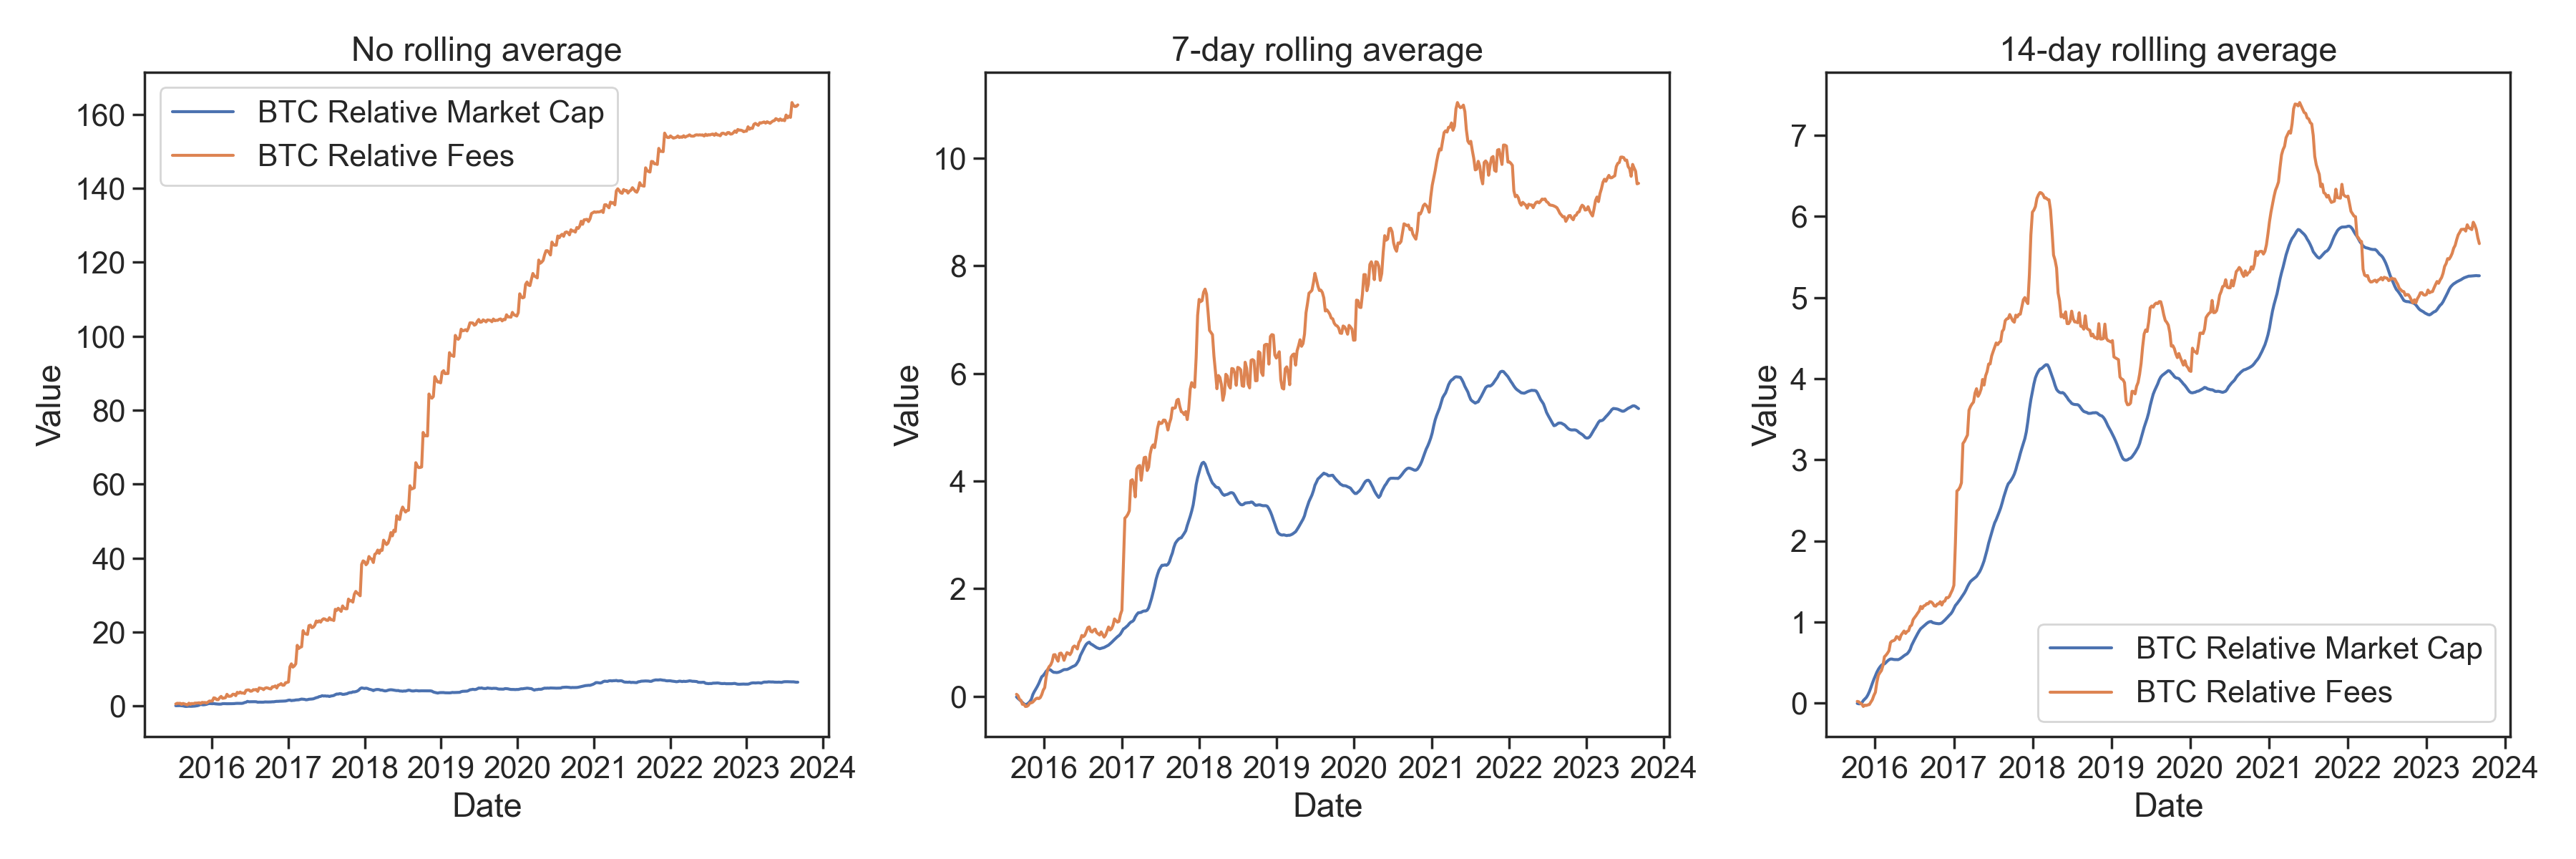
\includegraphics[scale=0.4]{figures/btc_avg_tx_fee.png}}
    \caption{Comparison of Relative variation in Bitcoin's transaction fees and market capitalization}
    \label{fig:comparison_fees_cap}
\end{figure}

The resulting factors were used to calculate the attribution share for each persona, using the hybrid attribution model. The results, along with the isolated Balance and Transaction models are presented in table \ref{tab:persona_emissions}.

\subsection{Attributed Emissions}


    \begin{table}[h]
    \centering
    \caption{Cumulative Attributed Emissions $C(t)$ (tC02e) for User Personas Using Passive (Assets), Active (Tx) and Hybrid allocations}
    \label{tab:persona_emissions}
    \centerline{
    
\begin{tabular}{lcccccc}
\toprule
\multirow{2}{*}{Persona Name} & \multicolumn{3}{c}{BTC} & \multicolumn{3}{c}{ETH} \\
\cmidrule(lr){2-4} \cmidrule(lr){5-7}
                                      & \textbf{Assets (t)}    & \textbf{Tx (t)}        & \textbf{Hybrid (t)} & \textbf{Assets (t)} & \textbf{Tx (t)} & \textbf{Hybrid (t)} \\
\midrule
Day Trader & $260$ & $1263$ & $1243$ & $697$ & $22$ & $38$ \\
Institutional Investor & $7514$ & $218$ & $364$ & $3204$ & $5$ & $81$ \\
Occasional User & $2$ & $22$ & $22$ & $0.63$ & $0.51$ & $0.51$ \\
Occasional User (2022) & $0.07$ & $5$ & $5$ & $<0.001$ & $<0.001$ & $<0.001$ \\
Retail Payment User & $15$ & $468$ & $459$ & $14$ & $8$ & $8$ \\
The Hodler & $137$ & $11$ & $13$ & $56$ & $0.2$ & $2$ \\
DAO Lending Protocol & -- & -- & -- & $1053$ & $63$ & $87$ \\
\bottomrule
\end{tabular}
}\end{table}



\begin{figure}[h!]
    \centering
    \centerline{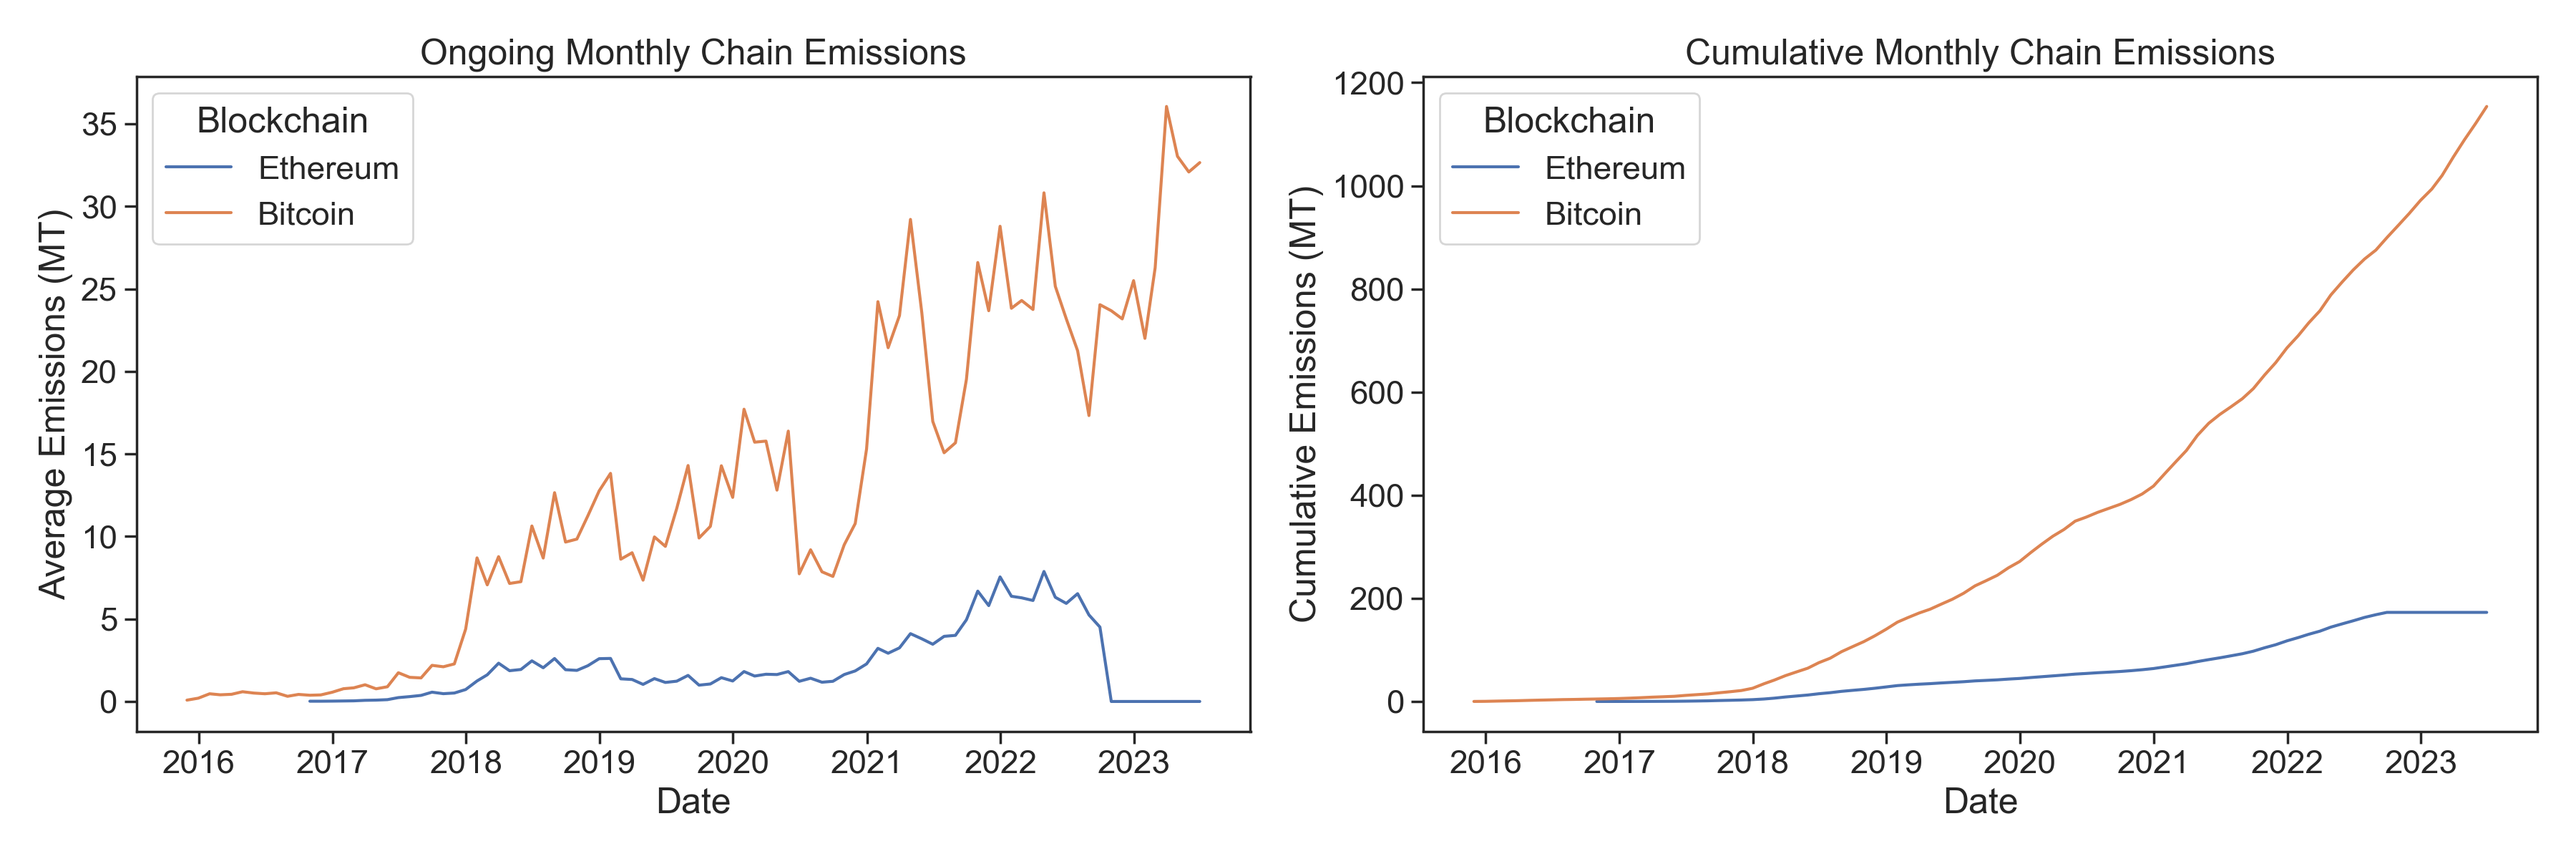
\includegraphics[scale=0.4]{figures/ongoing_cumulative_emissions.png}}
    \caption{Historical and Cumulative Emissions for the Bitcoin and Ethereum Networks}
    \label{fig:ongoing_emissions}
\end{figure}

Emissions numbers follow the hypotheseses established in the previous section. The bitcoin network personas show higher emissions attributed accross the board. The only exception being the day trader, whose modelized investing behavior better payed off in early years than bitcoin at the same time. We see that the regular transactions of the retail payment user leads to important emissions reaching 468 tCO2e for the transaction attribution, while balance attribution stays low. Finally, the most recent user still gets attributed relatively important transaction emissions (5t) considering its moderate 10 interactions, this is many orders of magnitude superiod to emissions of the user on Ethereum-PoS ($\tilde{0.2kg}$). And is in line with the reported reduction of electricity consumption on the network since the transition to PoS.

Figure \ref{fig:ongoing_emissions} show historical and cumulative emissions reported by CCRI for both networks. The drop in emissions for the Ethereum chain is clear following 2022 and consistent with the litterature. Also consistent with the litterature is the post-2021 rapid increase in emissions for the Bitcoin network, caused by a significant reduction in miners relying on renewable energy sources. This may explain why the even the recent occasional bitcoin user is attributed the equalivalent of five New-York Paris flights worth of emissions for anectotal interaction with the system. Figure \ref{fig:attributed_investor} also show similar pattern, where we see an acceleration of attributed emissions for the institutional investor as the token price drops and he is able to acquire more for the same dollar investment. This is raising concerns, as at the same time the value of the network has dropped significantly. Thus counted in emissions per unit of value delivering, the network in increasingly going in the wrong direction. Historical emissions for the other personas are presented in appendix \ref{appendix:historical_emissions}.


\begin{figure}[h!]
    \centering
    \centerline{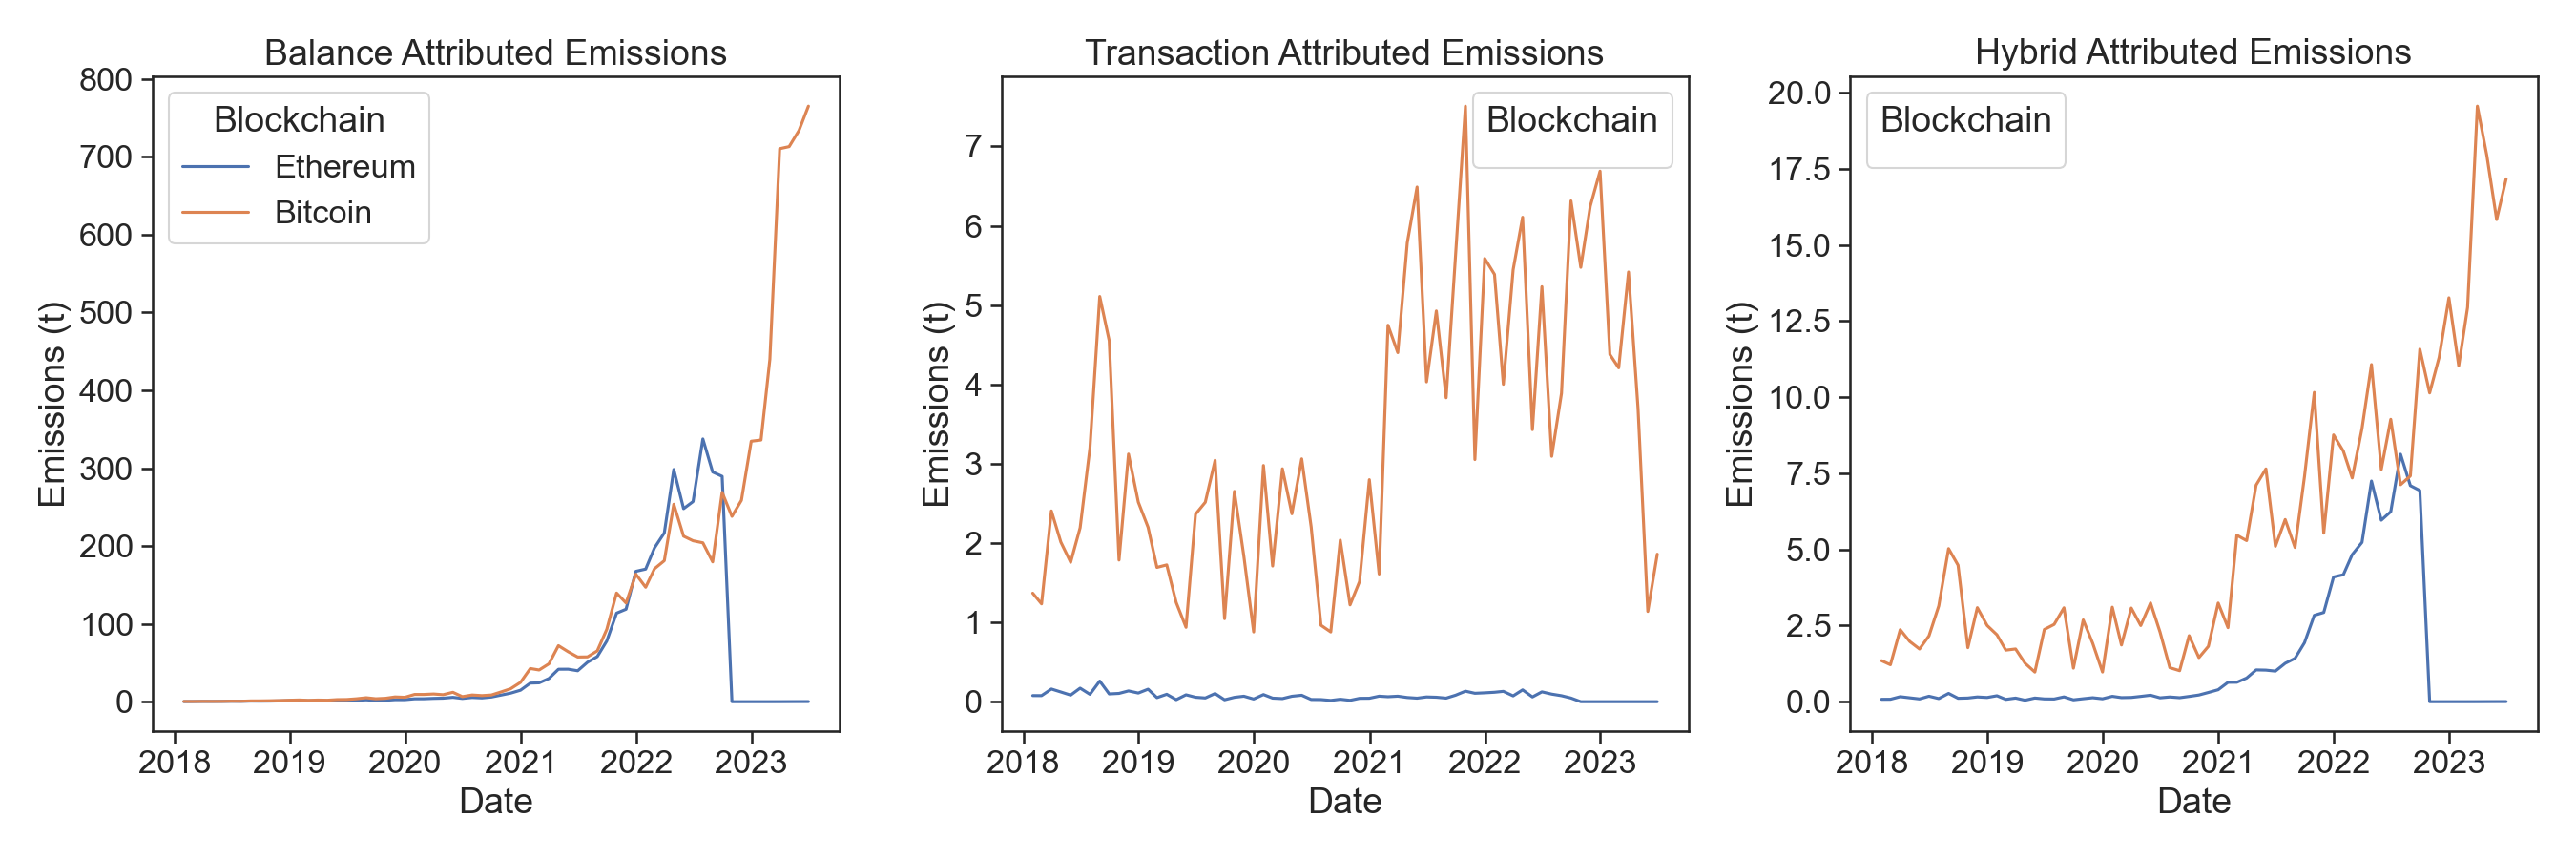
\includegraphics[scale=0.4]{figures/attributed_em_invest.png}}
    \caption{Historical Attributed Emissions for the Institional Investor}
    \label{fig:attributed_investor}
\end{figure}


\begin{figure}[h!]
    \centering
    \centerline{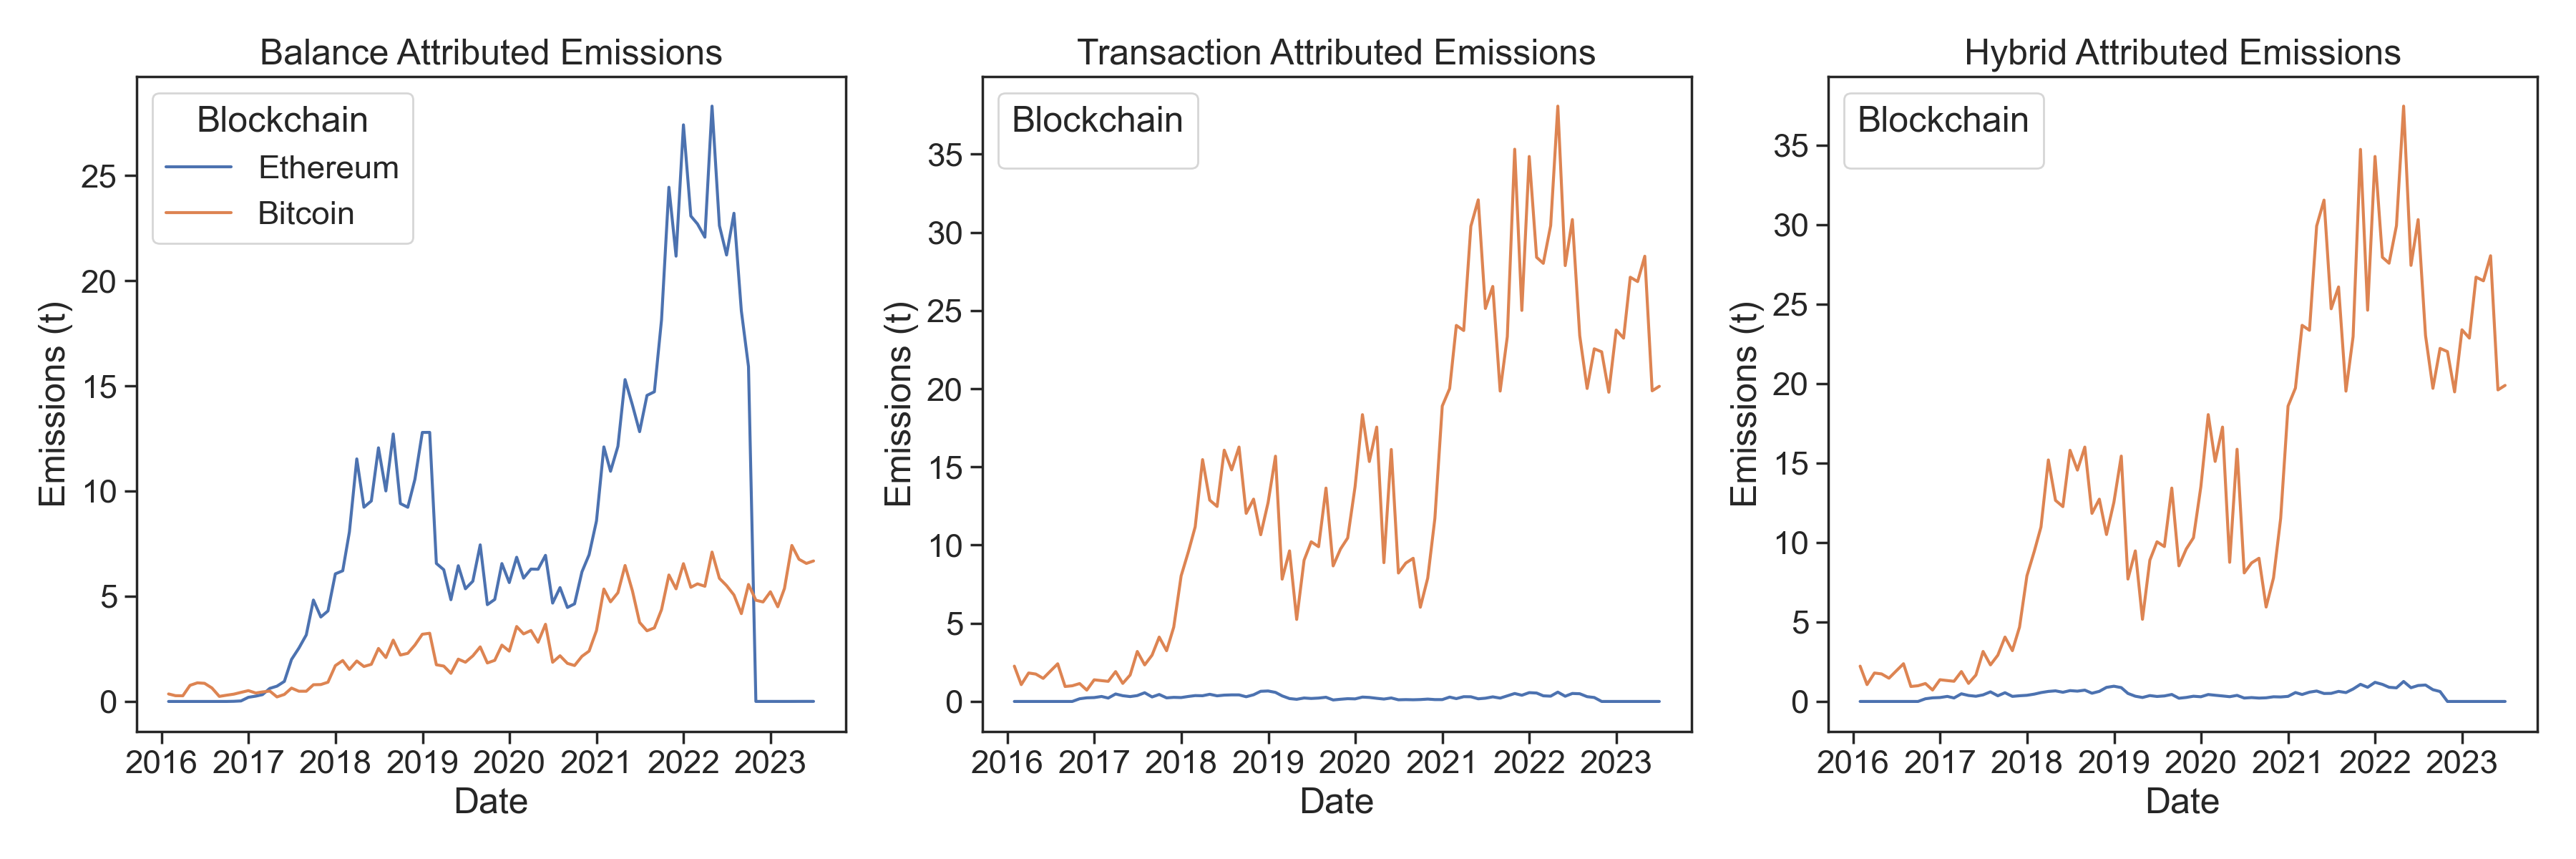
\includegraphics[scale=0.4]{figures/attributed_em_trader.png}}
    \caption{Historical Attributed Emissions for the Day Trader}
    \label{fig:attributed_trader}
\end{figure}


\subsection{Industry \& Academia Expert Interviews}\todo{TODO}

Interviews were conducted with experts across industry and academia working at the intersection of blockchain and sustainability. The goal was to receive feedback on the research methodology and learn about relevant work that could inform the thesis.

Discussions focused on areas for improvement in the methodology, data access \& collection, and potential use cases for the Greenblocks platform. The following experts were interviewed:

\begin{enumerate}
    \item Maria Eisner Pelch, Senior Sustainability Manager at Concordium - A novel blockchain project enabling sustainability use cases like tradable green energy certificates. She provided perspective on blockchain partnerships with government entities in the sector of energy. She was was critical of work by the CCRI.
    \item Marcus Aurelius, CTO and Core Contributor of KlimaDAO - Integration with the Klima on-chain volontary carbon market is a core Greenblocks component. The discussion helped answer methodology questions and specifics around integrating with their platform.
    \item Loic Leray, Sustainability Consultant for DeepSquare - A Swiss blockchain startup offering decentralized sustainable computing. We discussed lifecycle analysis processes and potential for blockchain footprinting at the user level.
    \item Alex de Vries, Researcher and PhD Candidate at VU Amsterdam - Authored influential blockchain sustainability papers and collaborated in the past with CCRI. Expressed disapproval of CCRI's hybrid attribution approach, that is partly based on his work, and noted industry pressure to average down per-transaction emission numbers.
\end{enumerate}


\chapter{Discussion}

\section{Selection of the Attribution Model for GreenBlocks}

Following analysis of the results and in accordance with expert interviews conducted, the hybrid attribution model was found inferior to the usage of both balance and transaction-based model in parallel. CCRI's still opaque methodology at attempting to fix the weight did not convince experts in the field nor does it is available right now to be used by the proof-of-concept. Since it applies chain specific methodologies to set the hybrid weights. Modeling user intent is feasible but prone to uncertainty and arbitrary opinionated decisions.

\section{Limitations}

\subsection*{Using proportional benefits as a proxy for emissions responsibility}
The \textit{Beneficiary Pays} approach, which analyses proportional benefits, has to be limited in its scope to be applicable. The complexity in this method scales exponentially because, for each horizontal use case, we find a collection of sub-benefits that could be weighted against each other to get the most exhaustive representation of user benefits. In this research, we stayed at the first level of abstraction, only considering that the number of transactions (or gas spent) as a share of the network total was indicative of benefit to the end user. However, for instance, one could argue that the transaction use case of blockchains should be weighted more granularly, being different for each transaction. One way to measure this benefit could be to look at transactional volume or fees paid by the user (as a share of the total for a period). Account holdings on GPCs could also be analyzed in a similar differentiated fashion. This would require a more granular data collection and analysis but could be a valuable addition to the model.
\improvement{link to future work and dealing with more complex behavioral data}

\subsection*{Limited Number of Attribution Parameters}
The model focuses on two main attribution parameters, inferred from emissions causality pathways and benefits rendered to the user, \textit{asset balance} and \textit{transactional activity}, each weighed by factors that represent how much each parameter should contribute to overall emission attribution (see \ref{se:methodology_overview} Methodology Overview). A more granular separation of the sub-benefits could be conducted to derive more attribution parameters. However, it would require nested-multiplied data modeling to estimate weight factors for each sub-benefits included in the formula. Moreover, since the hybrid approach was not chosen to combine all attribution factors in a single footprint number, a decision was made to keep high-level parameters (2) and report these two numbers to the user.


\subsection*{Weighting Factor Uncertainty}
Using average relative changes over long intervals may fail to capture more nuanced shifts in user priorities over shorter timescales. The limits to this approach was also show when discussing weight factor results, as an artitrary decision of moving average had to be made, with significant impact on the weights value. This approach also assumes user behaviors are consistent across all blockchain users, whereas, in reality, different segments likely have distinct preferences. These limitations are discussed further in Section \ref{se:limitations}.


\subsection*{Single Network Personas}





\chapter{Implementation: GreenBlocks Platform}
\section{Overview \label{se:implementation_overview}}
\begin{figure}[h!]
    \centering
    \centerline{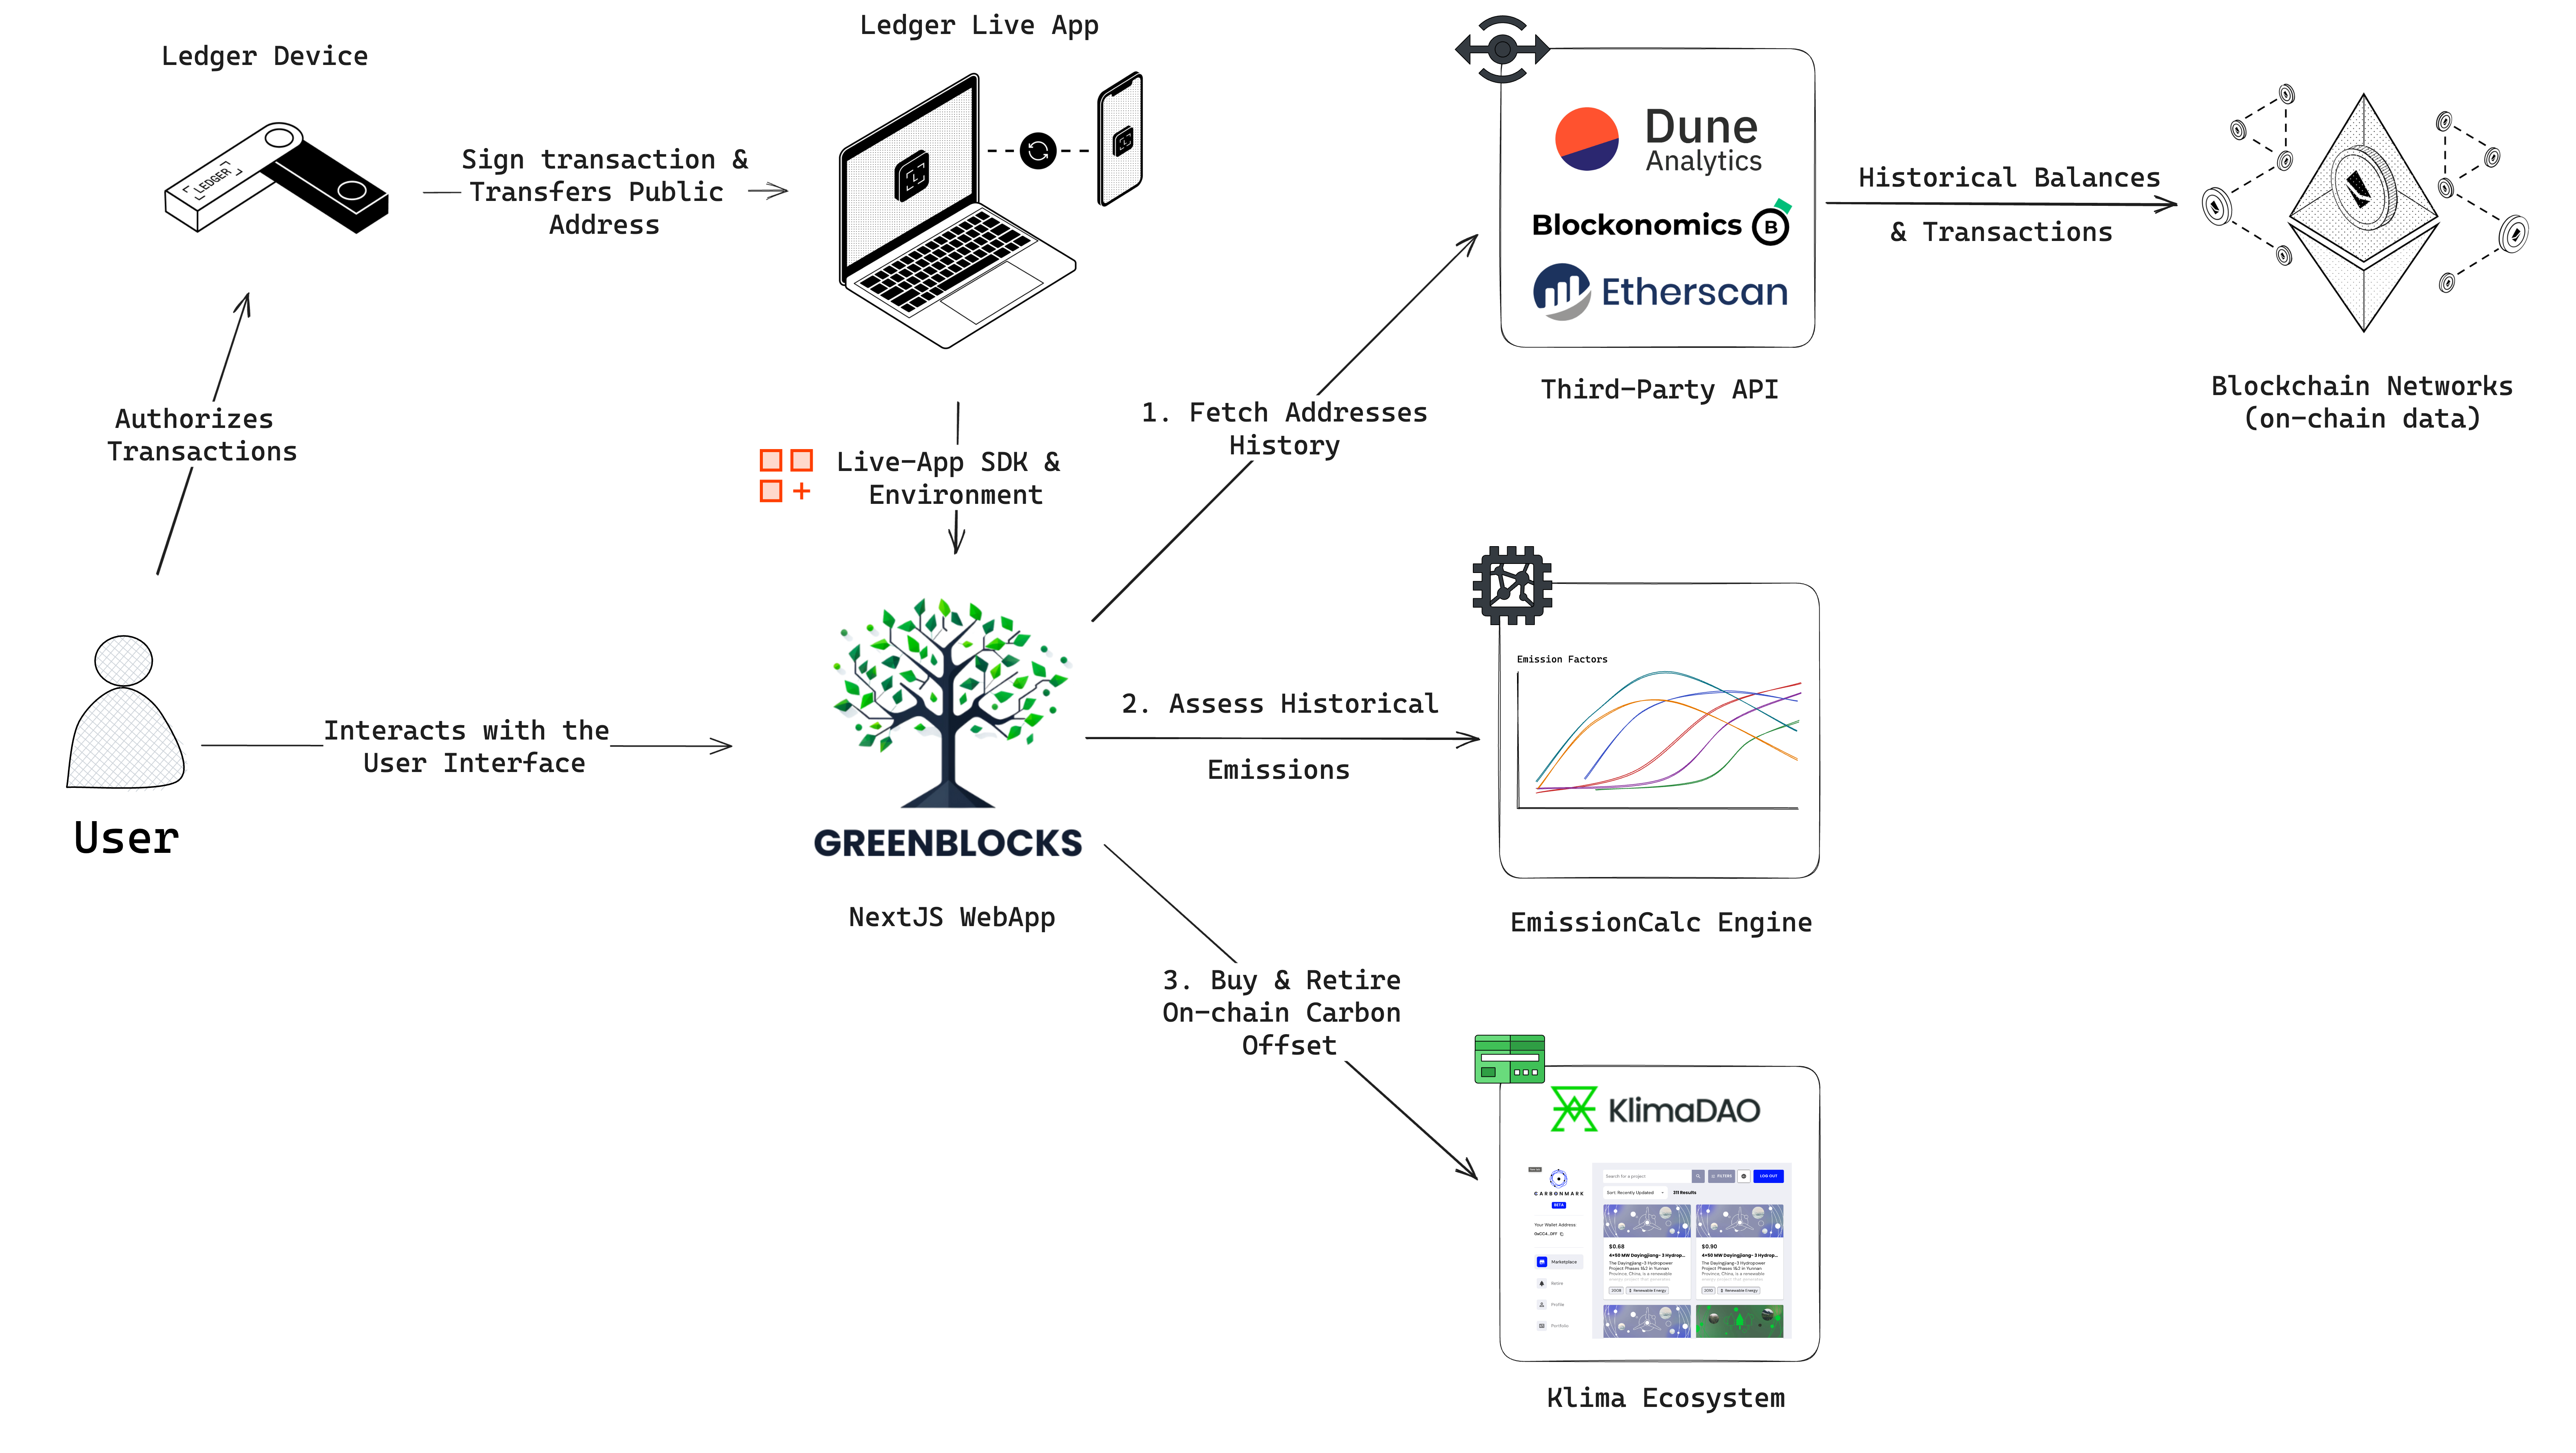
\includegraphics[scale=0.08]{figures/functionnal architecture.png}}
    \caption{GreenBlocks - Functionnal Architecture}
    \label{fig:functionnal_architecture}
\end{figure}

\begin{figure}[hbt!]
    \centering
    \centerline{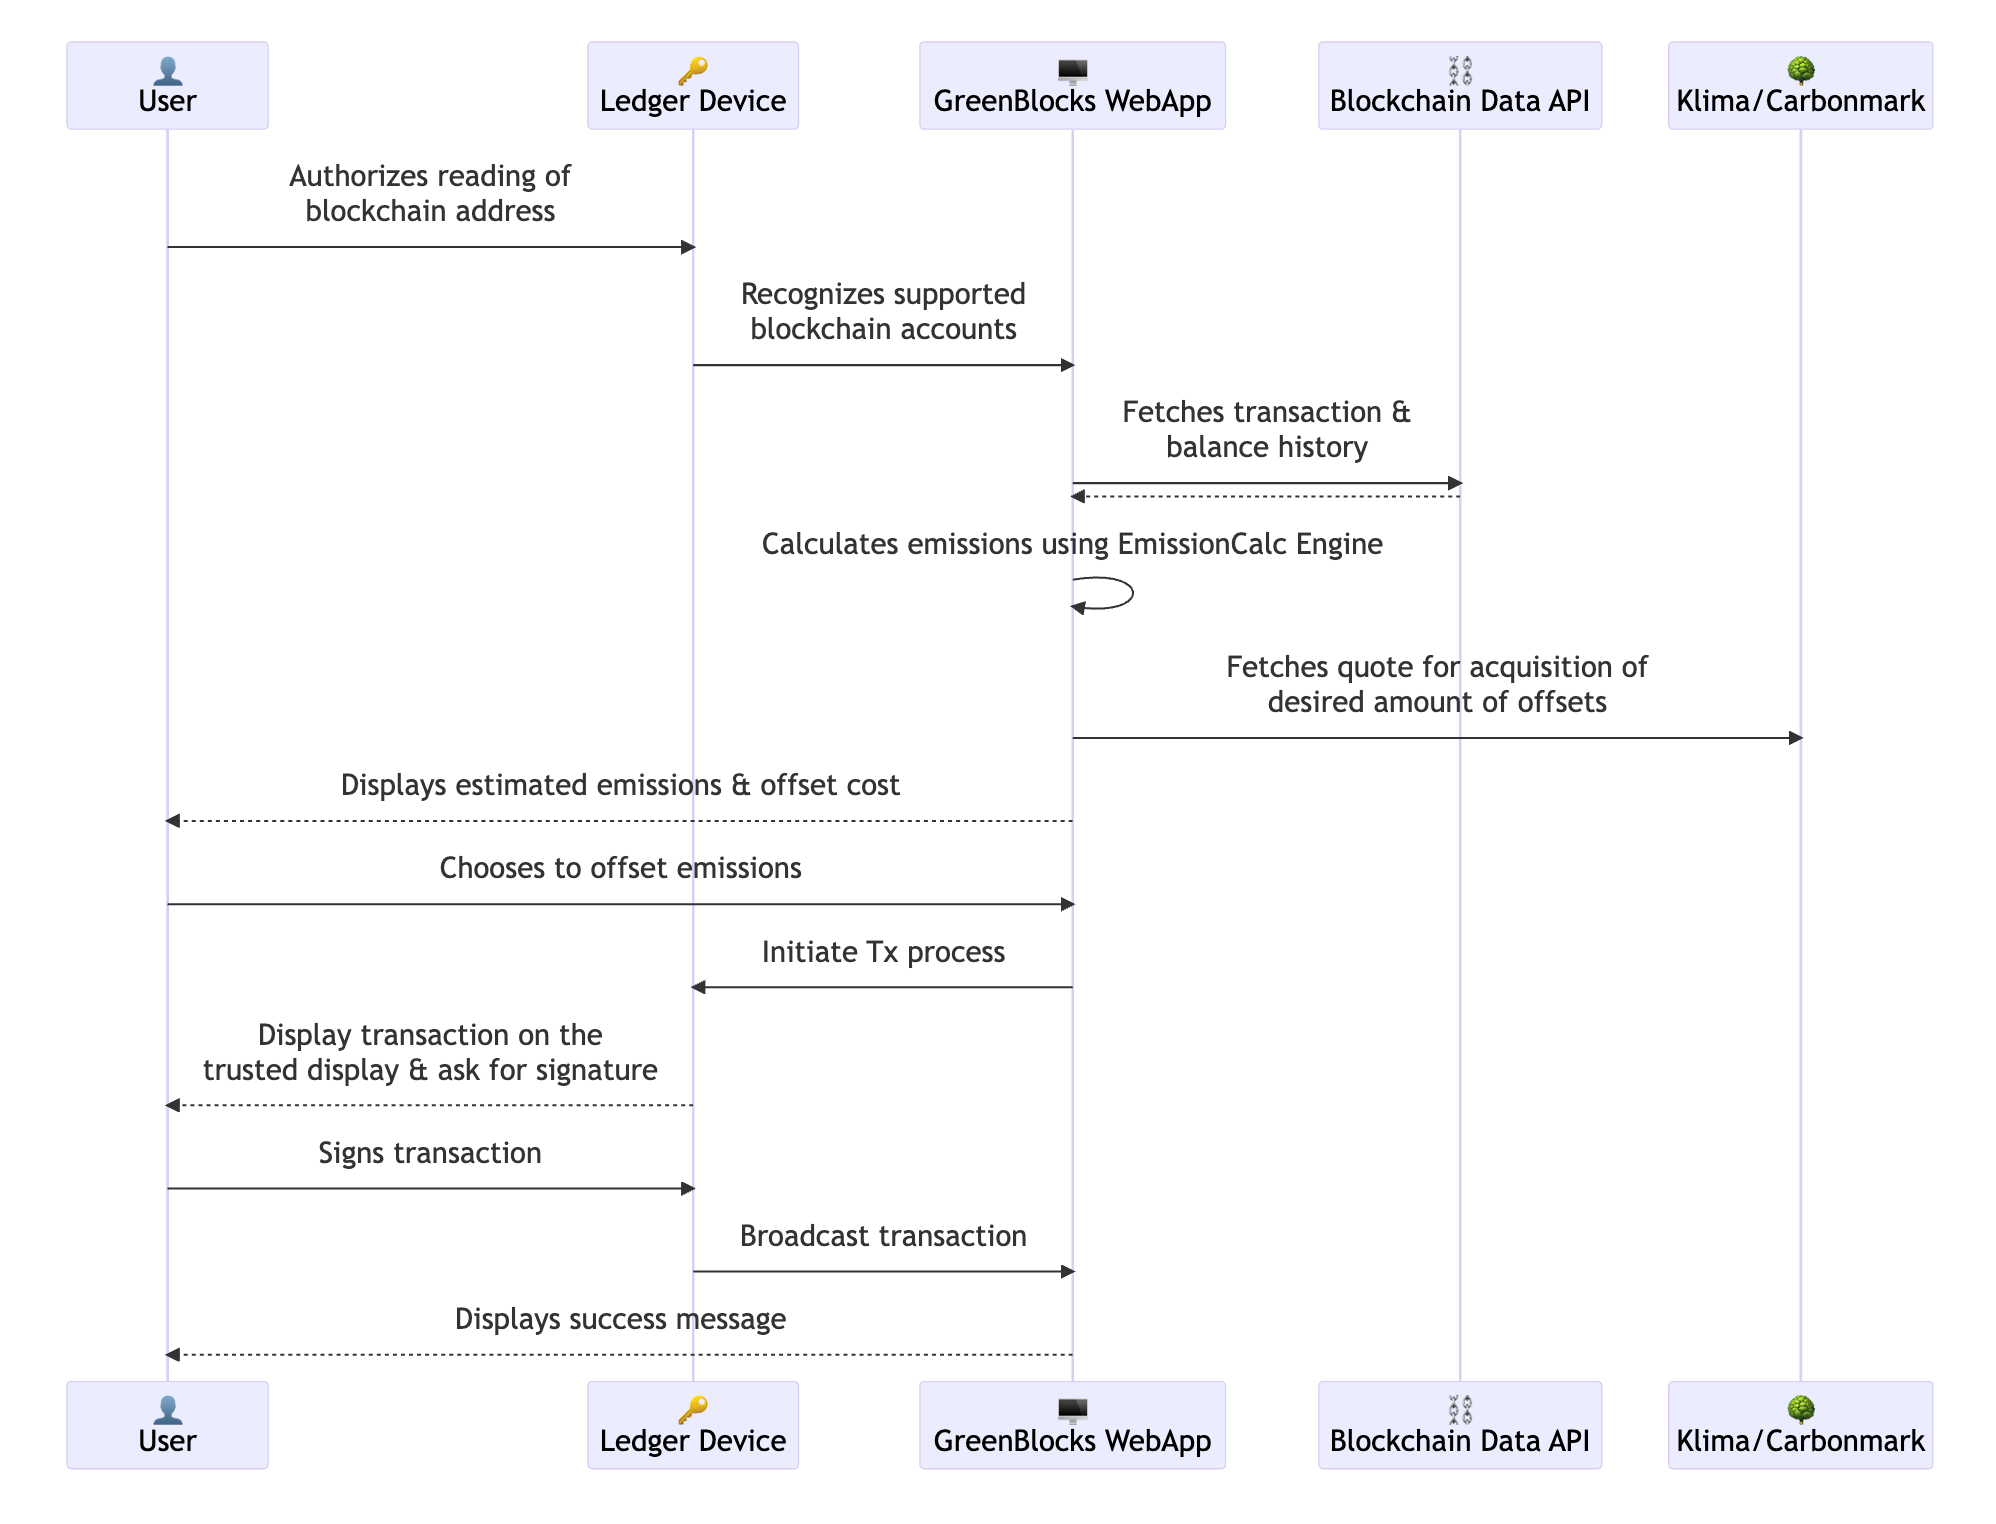
\includegraphics[scale=.27]{figures/sequence.png}}
    \caption{GreenBlocks - Sequence Diagram}
    \label{fig:sequence}
\end{figure}

\change{Review figure size for readability. Consider redo on lucid to control font}


\section{System Architecture and Components}
\subsection{User Interface Layer}
\subsection{Middleware Layer}
\subsection{Backend Layer}
\subsection{Data Layer}
\section{Development Process}




\newpage


\section{Limitations and Future Work} \label{se:limitations}
\section{Further Opportunities for Blockchain and Sustainability}

\chapter{Conclusion}

As blockchain technology expands onto more use cases and scales in its adoption, quantifying and attributing associated carbon emissions transparently emerges as a valid need. While aggregate estimates provide high-level network overviews, they fail to offer individual user-level accountability, posing a user education gap and potentially a product need.

\bibliography{bibliography.bib}

\newgeometry{textwidth=6in,textheight=10in}

\appendix
\titleformat{\chapter}[display]
{\normalfont\large\bfseries}% <- font for label "Appendix A", default \huge
{\chaptertitlename\ \thechapter}
{5pt}
{\large}% <- font for title, default \Huge

\chapter{User Personas Descriptions \label{appendix:user_personas_desc}}

\textbf{Day Trader}: Individuals who frequent buying and selling activities on Bitcoin and Ethereum networks. They are highly active and contribute to a significant number of transactions. They are usually first adopters or early followers and have been on the networks for several years.

\textbf{The Hodler}: Individuals who invest in cryptocurrency with a long-term perspective. They hold both Bitcoin and Ethereum and rarely engage in trading activities. These individuals are often early adopters of the technology and have held crypto assets for several years.

\textbf{Institutional Investor}: Large financial entities like hedge funds or mutual funds that make occasional but large transactions. They are relatively new to the cryptocurrency space compared to individual investors but hold significant assets in both Bitcoin and Ethereum.

\textbf{Retail Payment User}: Individuals using cryptocurrencies for regular small payments, such as online purchases or transferring money. They are active on Bitcoin and Ethereum networks and have used cryptocurrencies for a few years.

\textbf{DAO Lending Protocol}: This persona is specific to the Ethereum blockchain and primarily engages in smart contract interactions. Their behavior is characterized by a regular high amount of gas spent and a high average balance.

\textbf{Occasional User}: These individuals engage infrequently in the Bitcoin ecosystem. A low transaction count and a low average balance characterize their behavior. They are relatively new to the ecosystem.

\textbf{Occasional User (PoS)}: This persona showcases a user who onboarded the Ethereum network after transitioning to proof-of-stake in September 2022. As with the Bitcoin Occasional users, they are characterized by a low transaction count and a low average balance.

\newgeometry{textwidth=8.5in,textheight=7in}

\begin{landscape}
    \chapter{User Personas and Data Generation Strategies}
    \improvement{add specific numbers for generation strategies}
    \label{appendix:user_personas_table}
    \begin{table}[h]
        \centering
        \caption{Summary of User Personas and Data Generation Strategies for Ethereum and Bitcoin}
        \centerline{
            \begin{tabular}{|c|c|c|c|}
                \hline
                \textbf{Persona}       & \textbf{Blockchain} & \textbf{Initial Investment (USD)} & \textbf{Data Generation Strategy}                                                                                                                                                            \\
                \hline
                The Hodler             & Ethereum / Bitcoin  & 1000                              & \begin{tabular}[c]{@{}c@{}} Rare transactions.\\ Transaction frequency is Poisson-distributed (mean=0.1).\\ Transaction amount scaled by 0.02\% of current balance.\end{tabular}             \\
                \hline
                Day Trader             & Ethereum / Bitcoin  & 2000                              & \begin{tabular}[c]{@{}c@{}} Frequent trades.\\ Transaction frequency influenced by market volatility.\\ Transaction amount in USD (mean=50).\end{tabular}                                    \\
                \hline
                Institutional Investor & Ethereum / Bitcoin  & 25000                             & \begin{tabular}[c]{@{}c@{}} Infrequent but large transactions.\\ Frequency slightly influenced by market volatility.\\ Transaction amount scaled by 0.5-2\% of current balance.\end{tabular} \\
                \hline
                Retail Payment User    & Ethereum / Bitcoin  & 500                               & \begin{tabular}[c]{@{}c@{}} Uses mainly for retail payments.\\ Transaction frequency is Poisson-distributed (mean=3).\\ Transaction amount in USD (mean=5).\end{tabular}                     \\
                \hline
                DAO Lending Protocol   & Ethereum            & 20000                             & \begin{tabular}[c]{@{}c@{}} Regular contract interactions.\\ Transaction frequency is Poisson-distributed (mean=0.5).\\ Transaction amount in USD (mean=500).\end{tabular}                   \\
                \hline
                Occasional User (PoS)  & Ethereum            & 700                               & \begin{tabular}[c]{@{}c@{}} Rare transactions.\\ Transaction frequency is Poisson-distributed (mean=0.1).\\ Transaction amount in USD (mean=10).\end{tabular}                                \\
                \hline
            \end{tabular}
        }
    \end{table}
\end{landscape}

\newgeometry{textwidth=6in,textheight=10in}
\chapter{Historical Emissions for User Personas \label{appendix:historical_emissions}}

\begin{figure}[h!]
    \centering
    \centerline{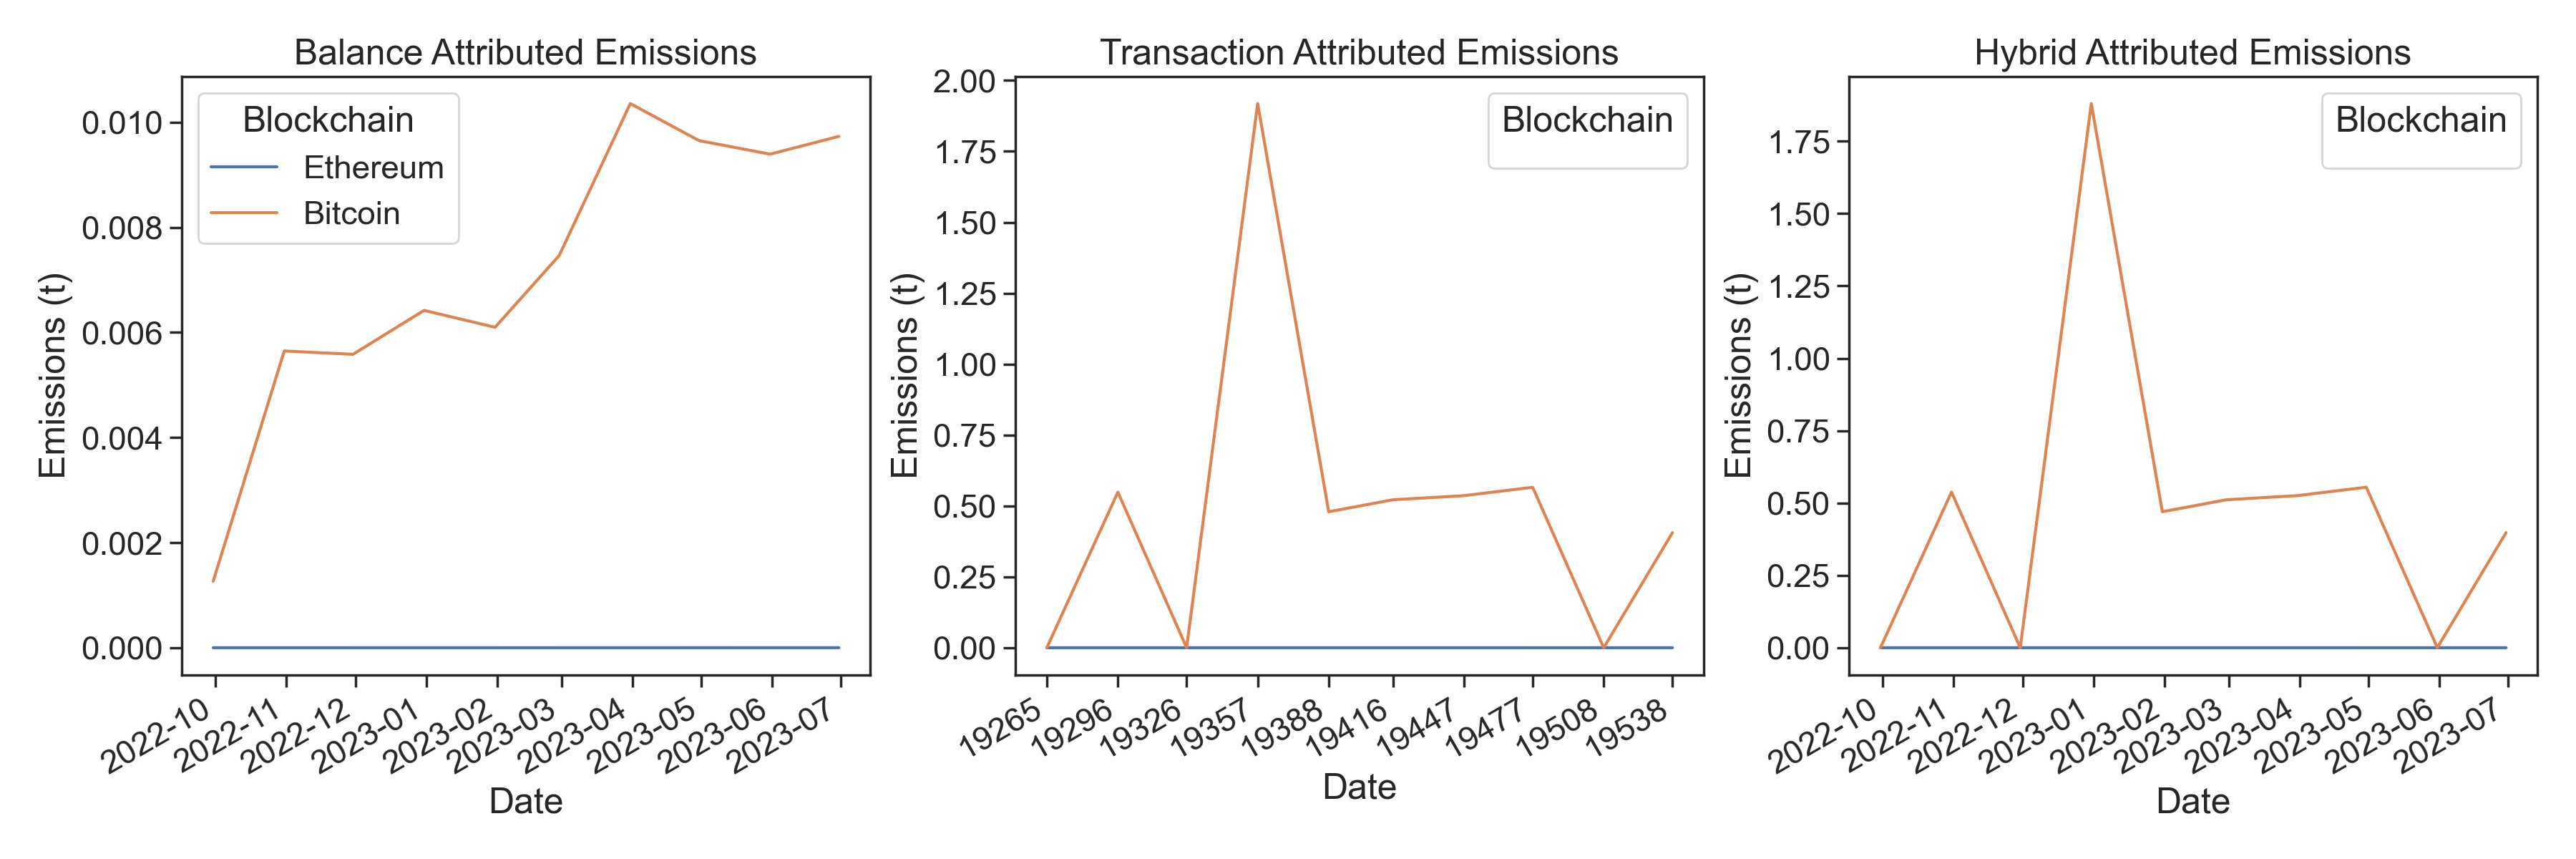
\includegraphics[scale=0.4]{figures/attributed_em_occasionaluser(2022).png}}
    \caption{Historical Attributed Emissions for the Institional Investor}
    \label{fig:attributed_investor}
\end{figure}
\begin{figure}[h!]
    \centering
    \centerline{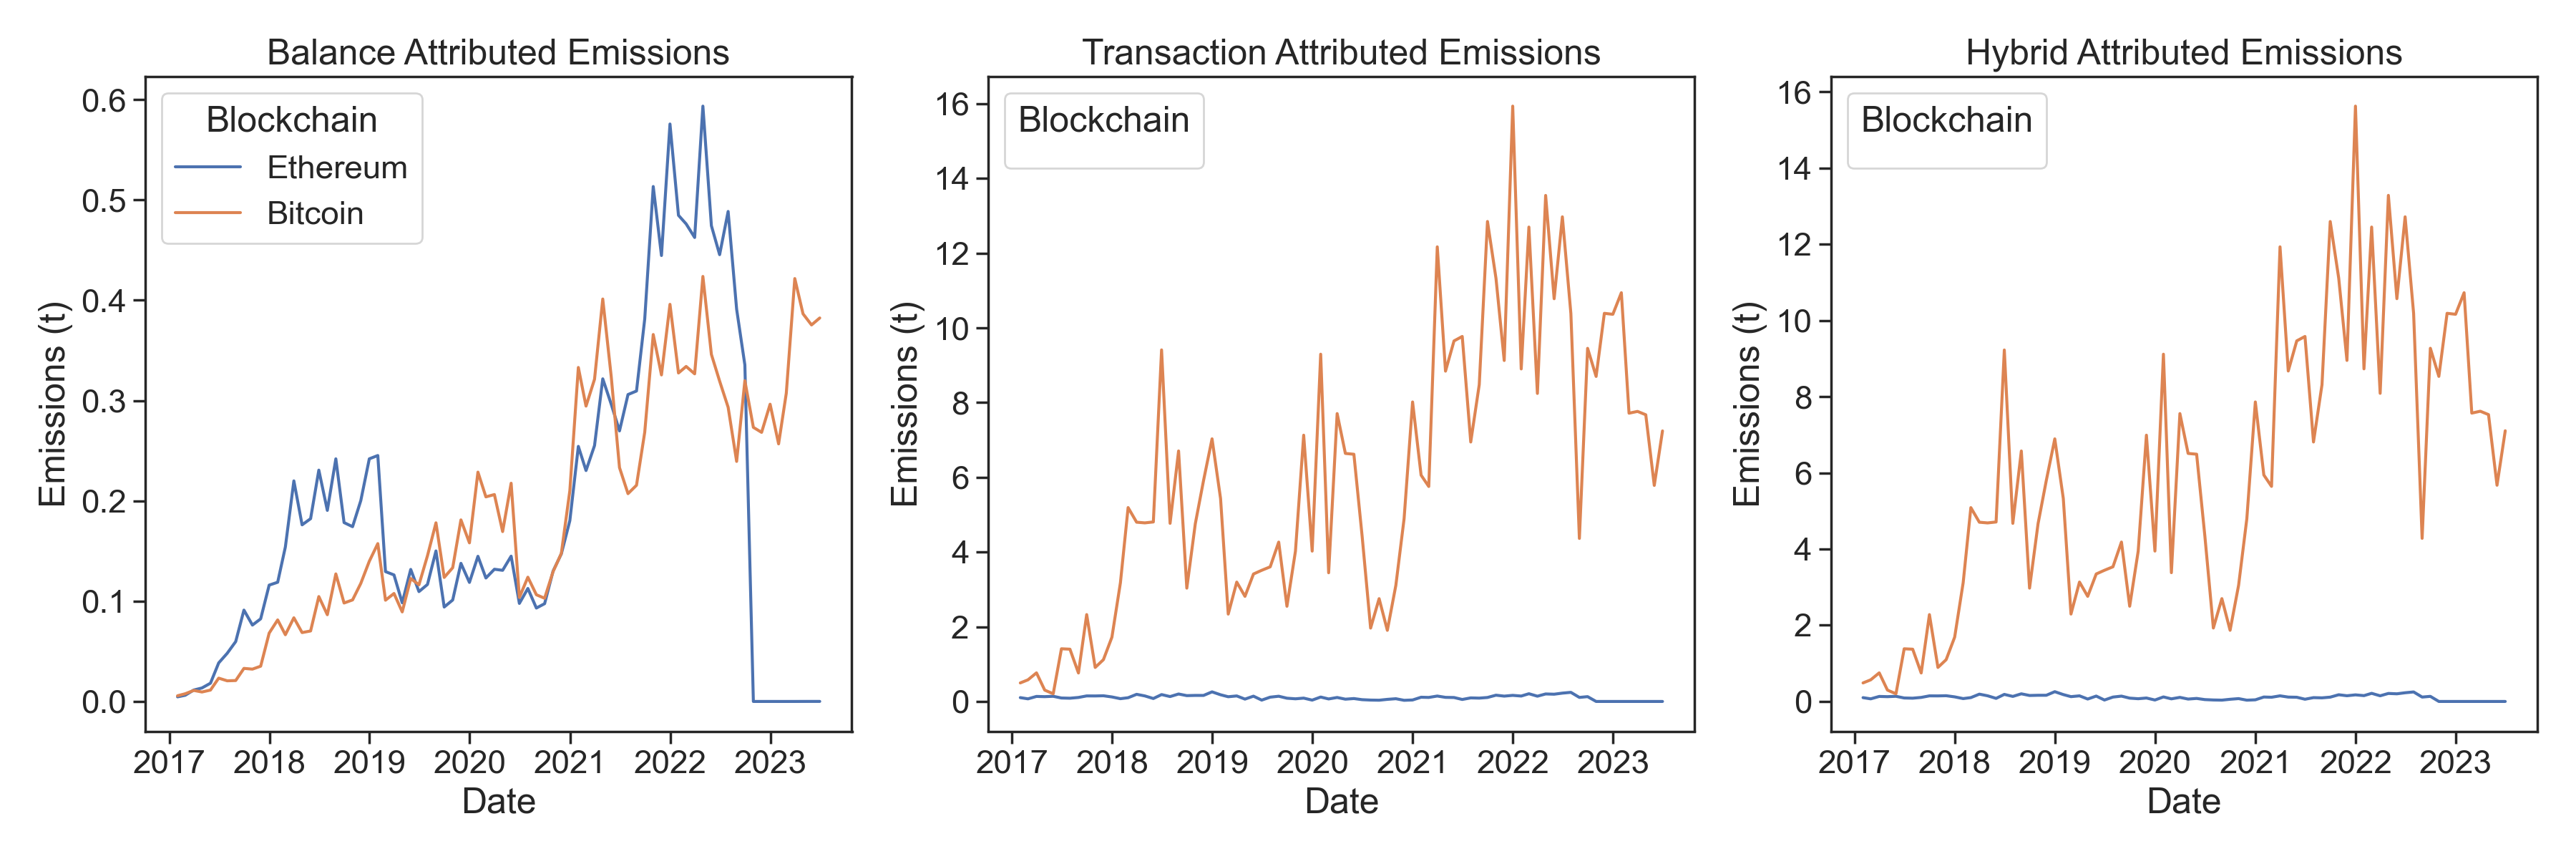
\includegraphics[scale=0.4]{figures/attributed_em_retailpaymentuser.png}}
    \caption{Historical Attributed Emissions for the Institional Investor}
    \label{fig:attributed_investor}
\end{figure}
\begin{figure}[h!]
    \centering
    \centerline{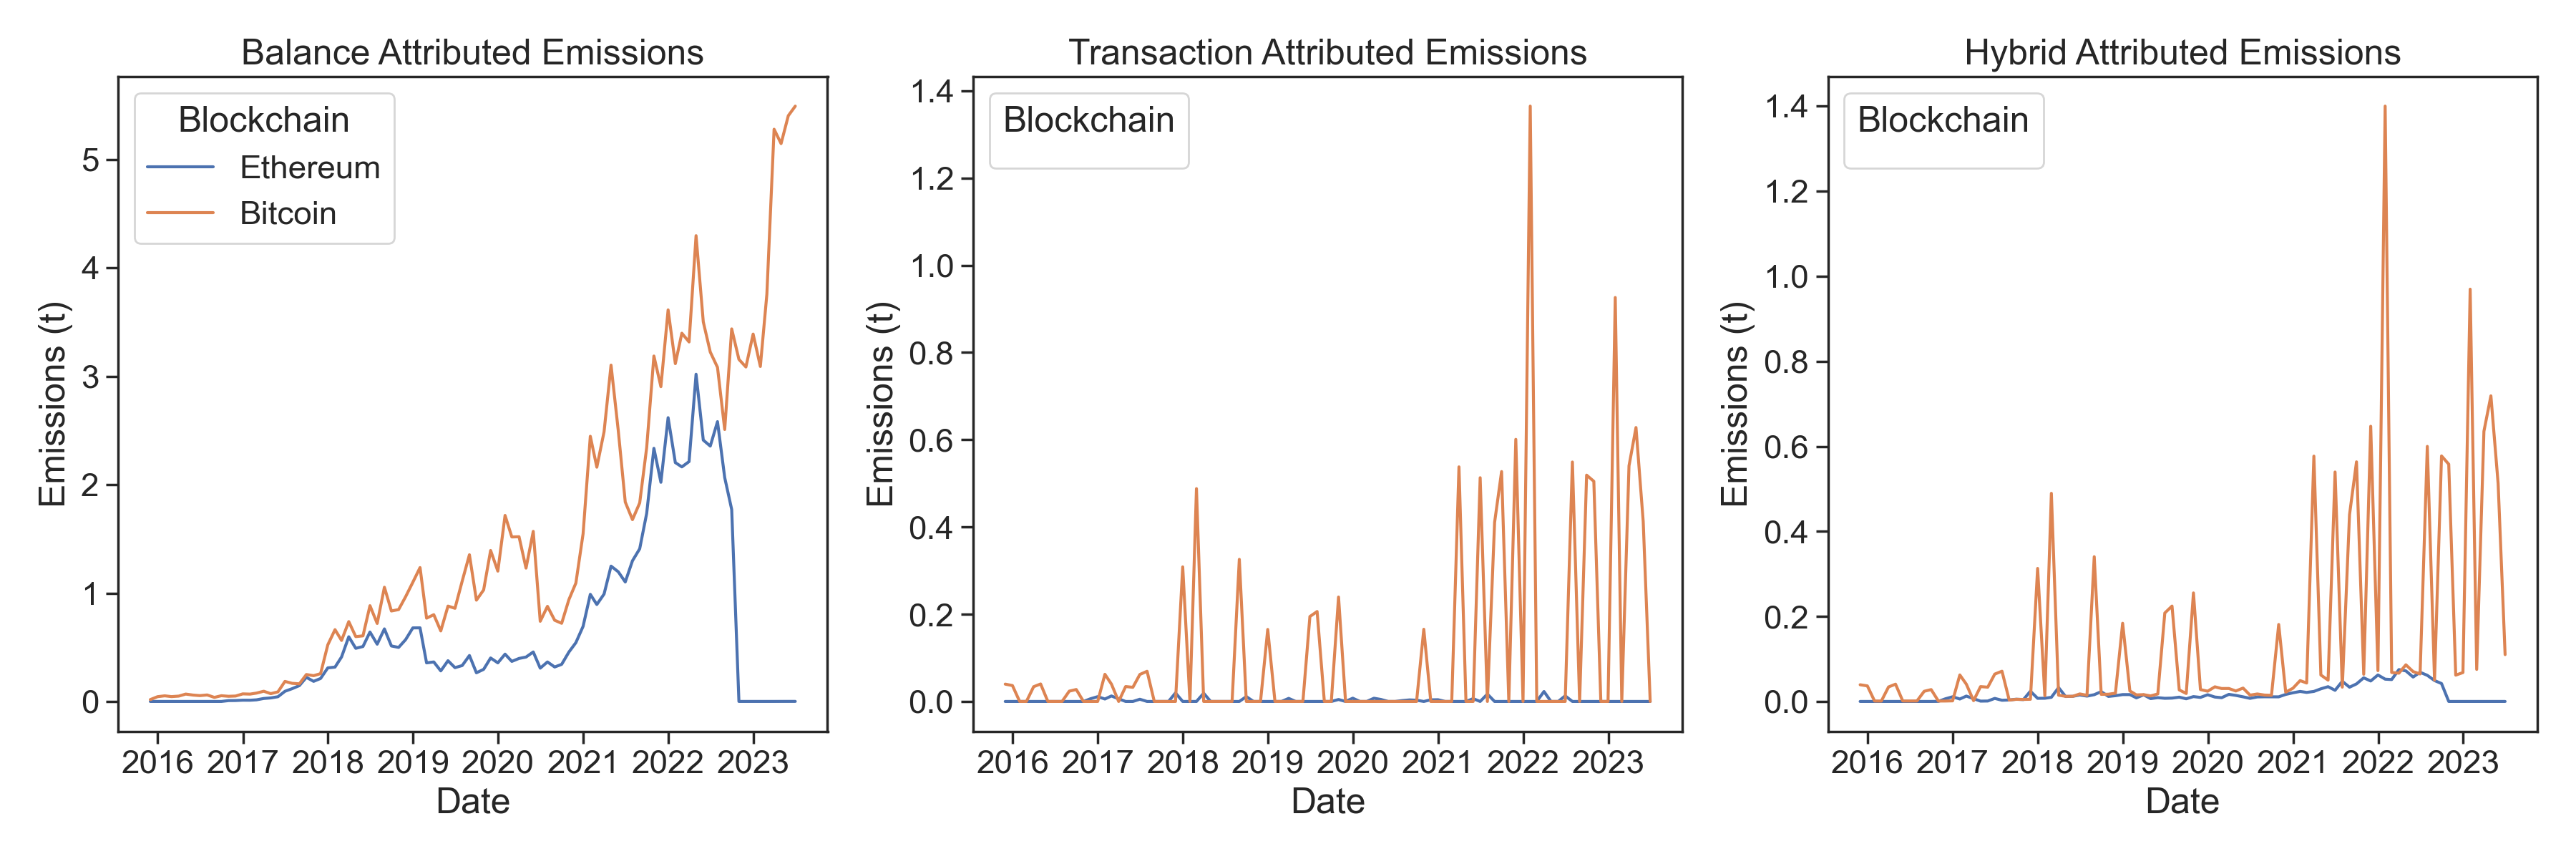
\includegraphics[scale=0.4]{figures/attributed_em_thehodler.png}}
    \caption{Historical Attributed Emissions for the Institional Investor}
    \label{fig:attributed_investor}
\end{figure}


\end{document}